%*****************************************
\chapter{Implementierung}\label{ch:implementation}
%*****************************************

Um die entwickelte Anwendung plattformübergreifend einsetzen zu können, wurde eine Angular-Single-Page-App mit ASP.NET-Back-End entwickelt. Dieses Kapitel beschreibt die Implementierung und die dabei genutzten Komponenten im Detail. Der Source-Code \cite{sourceCode} ist auf GitHub verfügbar

\section{Domain Model}

Das Domain Model besteht aus den in Abbildung \ref{fig:domModel} dargestellten Klassen. Dabei wird eine Messung durch Messdaten sowie zugehörige Metadaten, wie Name und Beschreibung, repräsentiert. Eine Messung kann entweder zu einer Zelle, einem Stack oder einem System gehören. Ein Stack ist eine Verschaltung von mehreren Zellen, ein System eine Verschaltung von mehreren Stacks. Systeme werden intern als Batteries bezeichnet, um Konflikte mit C\# Bibliotheken zu vermeiden. Die Enumeration \code{MeasurementType} beschreibt den Typ der Messung: Undefiniert, Zeitreihe, Ortskurve, oder Sonstige. \code{CircuitType} gibt die Schaltungsart an: Reihen- bzw. Parallelschaltung oder Sonstige. Neue Instanzen des jeweiligen Typs können zur Datenbank hinzugefügt, gelöscht, und bearbeitet werden. Es stehen jeweils List- und Detail-Views zur Verfügung. Die Messung hat eine Upload- und eine Download-Methode.

\begin{figure}
\centering
\makebox[\textwidth][c]{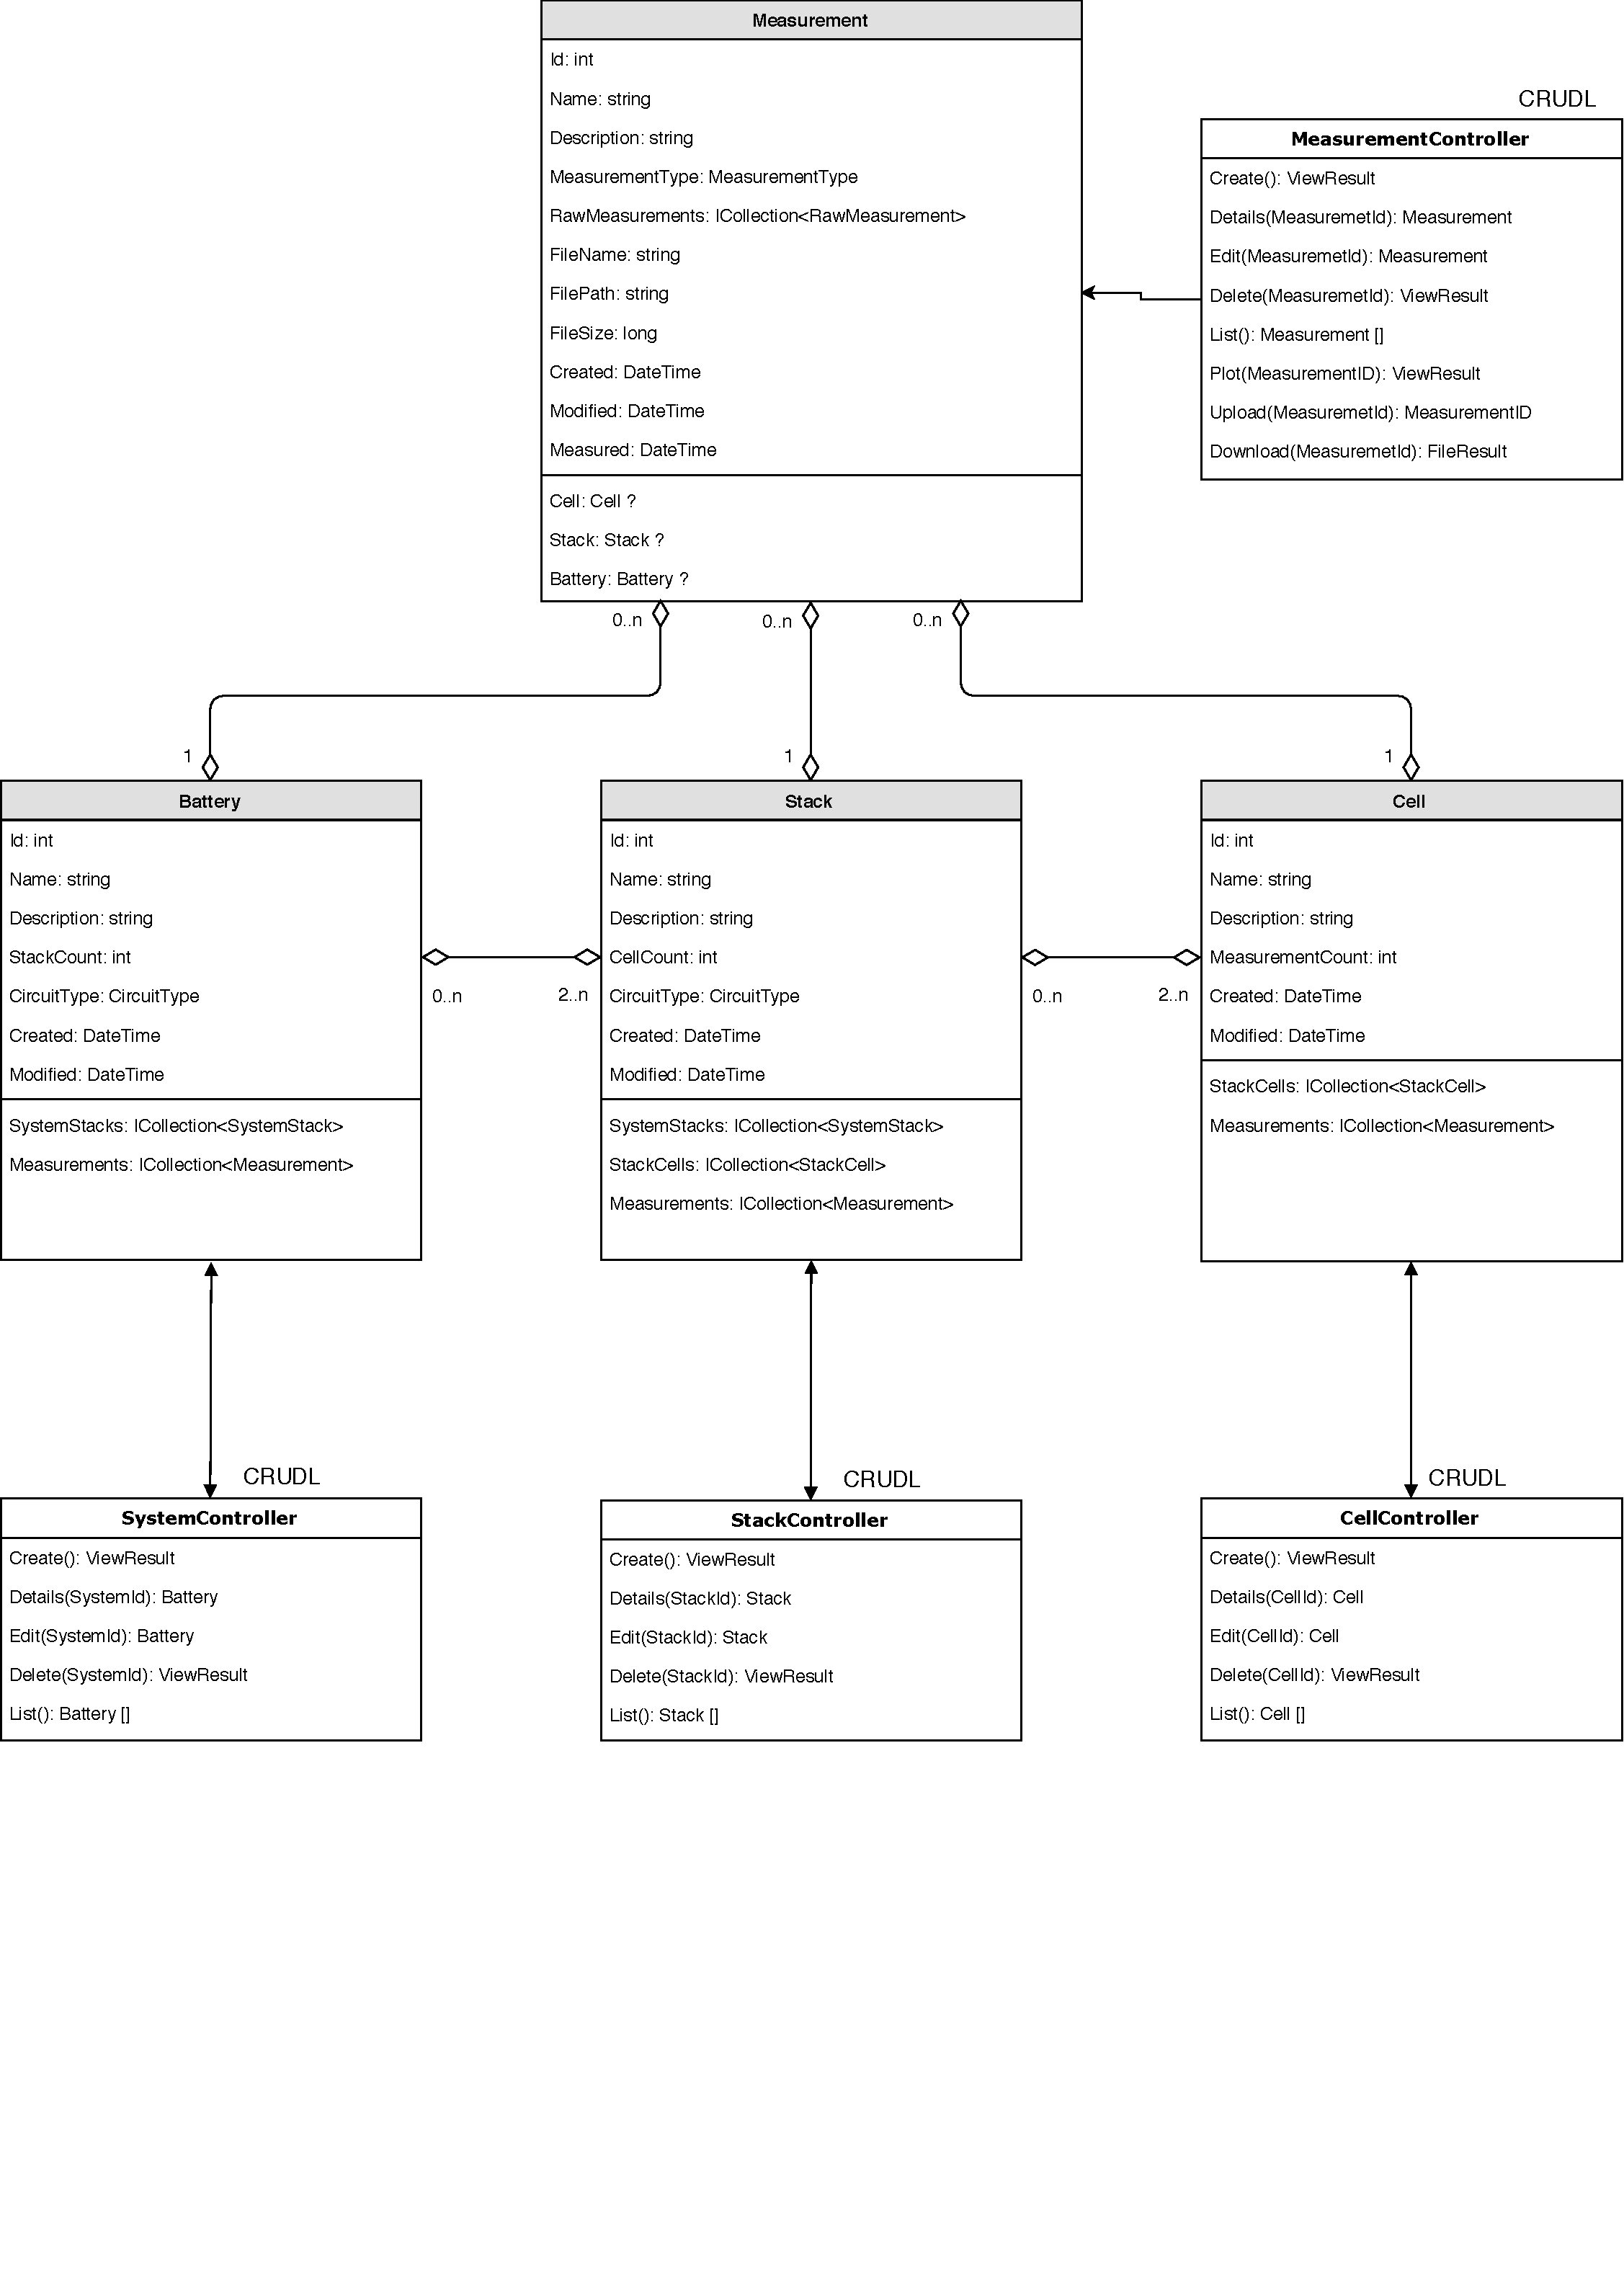
\includegraphics[width=1.4\textwidth]{Figures/classDiagram}}
\caption{Domain Model als UML Klassenhierarchie}
\label{fig:domModel}
\end{figure}

Abbildung \ref{fig:routing} zeigt die entwickelten Angular-Components und das Routing. Die Components werden weiter unten näher beschrieben.

\begin{figure}
\centering
\makebox[\textwidth][c]{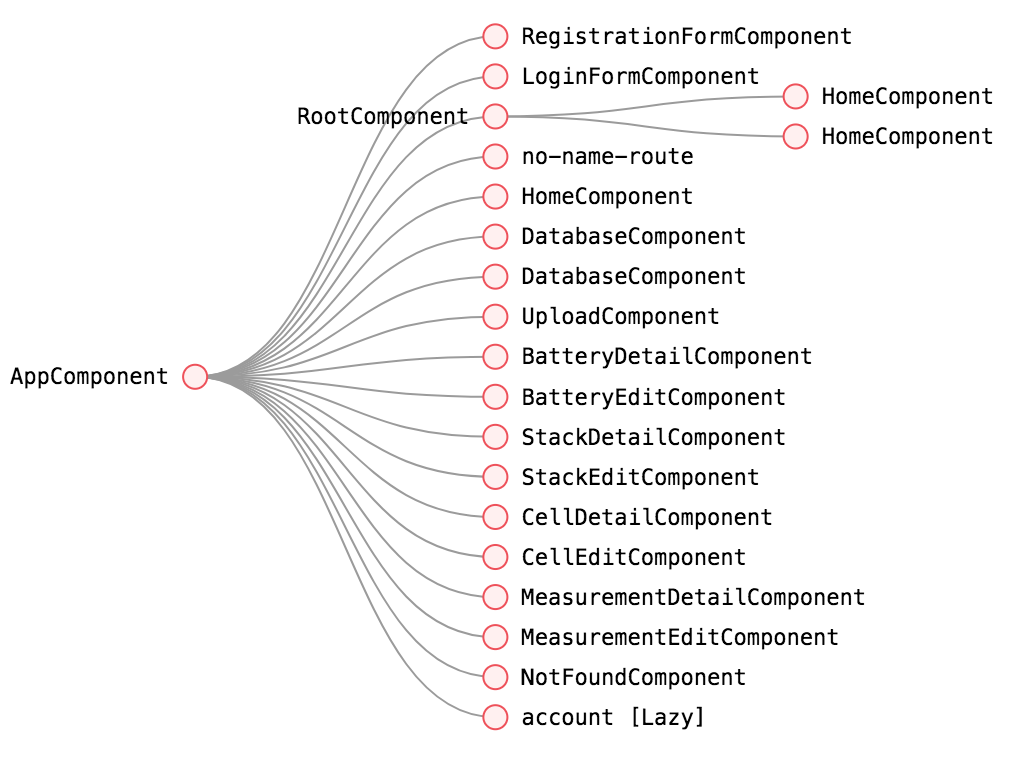
\includegraphics[width=\textwidth]{Figures/routing}}
\caption{Angular-Components und Routing}
\label{fig:routing}
\end{figure}


\section{Frameworks und Technologien}

Im Folgenden werden die verwendeten Frameworks und Technologien näher beschrieben.

\subsection{Angular}

Angular 4.x \cite{angular} ist ein TypeScript-basiertes Frontend-Webframework. Angeführt durch Google, wird es von einer Community aus Einzelpersonen und Unternehmen entwickelt und als Open-Source-Software über GitHub \cite{angularGit} publiziert.


\subsection{ASP.NET Core}

Die General-Purpose-Development-Platform .NET Core wird unter der Koordination von Microsoft zusammen mit der .NET Community entwickelt und ist als Open Source-Projekt über GitHub \cite{dotnetcore} verfügbar. Sie bietet eine platformübergreifende Lösung zur Entwicklung und Ausführung von Anwendungsprogrammen und läuft unter Windows, macOS and Linux. ASP.NET steht für Active Server Pages .NET und ist ein Web Application Framework von Microsoft, mit dem sich dynamische Webseiten, Webanwendungen und Webservices in C\# entwickeln lassen. Im Hintergrund läuft der Kestrel Web Server für ASP.NET \cite{kestrel}. Als Entwicklungsumgebung wurde Visual Studio Code mit C\#-Extension genutzt, ein kostenloser und quelloffener Texteditor.


\subsection{Entity Framework Core}

Entity Framework Core ist eine abgespeckte, erweiterbare, platformübergreifende Version des bekannten Entity Frameworks, ein Framework für objektrelationale Abbildung von Microsoft. Entity Framework Core ermöglicht es ausschließlich unter Benutzung von .NET-Objekten mit Datenbanken zu arbeiten und beseitigt so die Notwendigkeit eigenen Code zum Zugriff auf die Datenbank zu schreiben \cite{msentitiyframework}. EF Core verwendet das aus Entity-Klassen bestehende C\#-Domain-Model um daraus mit Hilfe von Migrations eine Datenbank zu erstellen. So kann das Domain Model während der Entwicklung einfach erweitert oder geändert werden, ohne händisch SQL-Befehle schreiben und testen zu müssen. Ein Datenzugriff auf eine Instanz einer Entity-Klasse wird durch Language Integrated Queries (LINQ) beschrieben \cite{dotnetcore}.


\subsection{SQLite}

SQLite implementiert eine eigenständige, serverlose SQL-Database-Engine und ist dabei die weltweit meistverwendete ihrer Art \cite{sqlite}. Anders als die meisten anderen SQL Datenbanken schreibt und liest SQLite direkt in und aus herkömmlichen Files auf einem Datenträger. Dabei ist das Fileformat platformübergreifend und frei kopierbar zwischen 32-bit und 64-bit Systemen sowie zwischen Big-Endian and Little-Endian Architekturen.


\subsection{Bootstrap und Now UI Kit}

Bootstrap \cite{bootstrap} ist ein freies CSS-Framework das responsive Webdesign vereinfacht. Es enthält auf HTML und CSS basierende Gestaltungsvorlagen für Typografie, Formulare, Buttons, Tabellen, Grid-Systeme, Navigations- und andere Oberflächengestaltungselemente. Bootstrap ist modular aufgebaut und besteht im Kern aus Less-Stylesheets. Als Erweiterung wurde das Now UI Kit \cite{nowUIkit} verwendet, was ein modernes, flaches und intuitives User Interface realisiert.

\subsection{Highcharts}

Highcharts \cite{highCharts} ist eine in pure JavaScript geschriebene Visualisierungslibrary der Firma Highsoft. Mit ihr lassen sich unter anderem interaktive Lineplots und Ortskurven erstellen. Auch lazy loading von Daten wird mit ihr vereinfacht.

\section{JSON-Fileformat}

Das JSON-Format wurde gewählt, weil es in C\# vorgefertigte JSON-to-Object Parser gibt und es flexibel und beliebig erweiterbar ist. Anders als beim ursprünglichen zum Logging genutzten CSV-Format, ist es einfach Metadaten und Zusatzinformationen zu speichern, ohne diese fest in gewissen Zeilen und Spalten zu kodieren. Weiterhin ist es menschenlesbar und portabel, anders als .mat-Files, die ursprünglich zur Speicherung der Ortskurven dienten. Listing \ref{lis:ortskurve} und \ref{lis:zeitreihe} zeigen jeweils die typische Struktur eines JSON-Files für eine Ortskurve und eine Zeitreihe mit beschreibenden Kommentaren.


\lstset{
	basicstyle=\small \ttfamily,
  breaklines=false,
  keepspaces=true, 
  language=Java,                 % the language of the code
  numbers=left,                    % where to put the line-numbers; possible values are (none, left, right)
  numbersep=5pt,                   % how far the line-numbers are from the code
  numberstyle=\tiny\color{gray}, % the style that is used for the line-numbers
  stepnumber=1,                    % the step between two line-numbers. If it's 1, each line will be numbered
  stringstyle=\color{red},     % string literal style
  caption={JSON Fileformat Ortskurven}                   % show the filename of files included with \lstinputlisting; also try caption instead of title
}

\lstinputlisting[label=lis:ortskurve]{Code/ortskurve.json}

\lstset{caption={JSON Fileformat Zeitreihen}}

\lstinputlisting[label=lis:zeitreihe]{Code/zeitreihe.json}

\section{REST API}

Representational State Transfer (REST) bezeichnet ein Programmierparadigma für verteilte Systeme, insbesondere Webservices. In einer Client-Server-Architektur stellt der Server einen Dienst bereit, der bei Bedarf vom Client angefragt werden kann. So stellt die REST API in unserer Single-Page-App Mess- und Metadaten aus der Datenbank bereit, die bei Bedarf dynamisch geladen bzw. nachgeladen werden.


\section{Zugriffsrechte}

Der Authentifizierung von Usern wurde mit Hilfe von JSON Web Tokes implementiert. Typisches Einsatzgebiet für JWT ist die fortlaufende Authentifizierung bei Single-sign-on. Da REST API’s zustandslos sind muss bei jeder Anfrage vom Client an den Server diese mit allen Informationen bestückt sein, die für die Verarbeitung der Anfrage benötigt wird. Damit man über die API Daten einsehen, hochladen, herunterladen und verändern kann, muss also immer ein vom Server zuvor generiertes JWT mitgesendet werden.


\chapter{Funktionalitäten} 

Nachfolgend ist ein möglicher Workflow beschrieben um die Funktionalitäten der App zu erläutern. Abbildung \ref{fig:home} zeigt den Home-View, der den Ausgangspunkt dafür bildet.

\begin{figure}
\centering
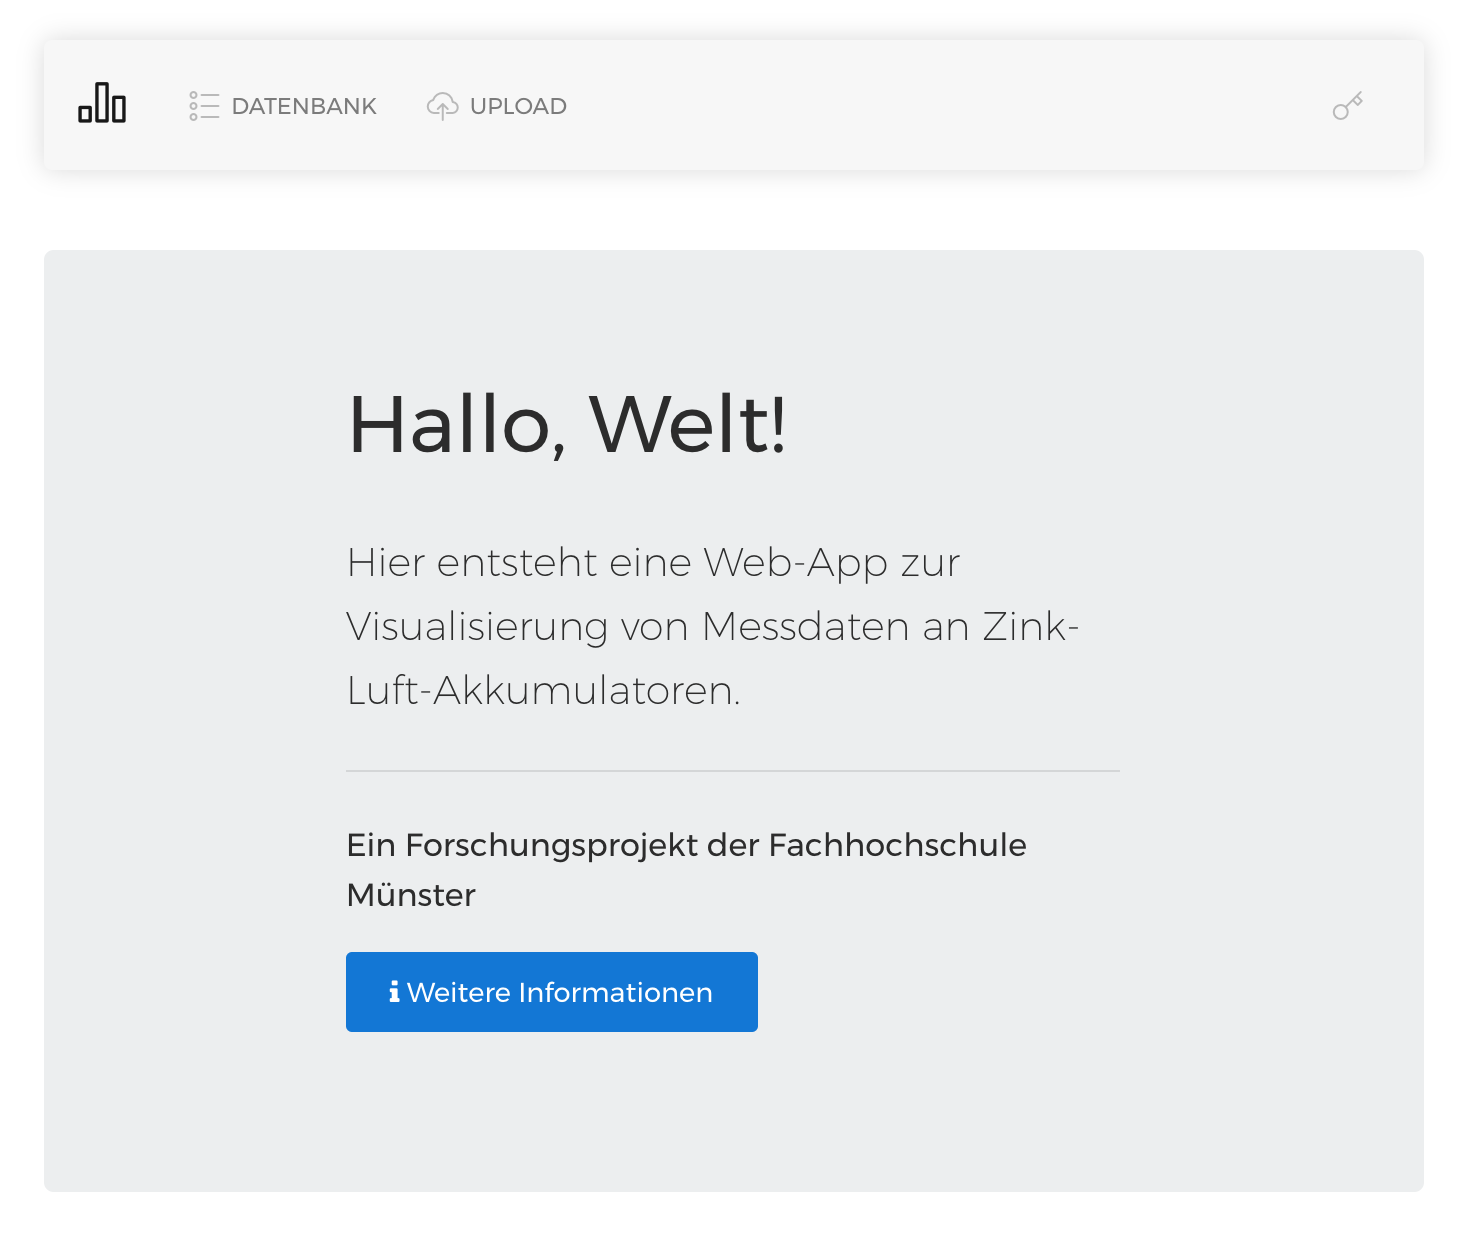
\includegraphics[width=\textwidth]{Figures/home}
\caption{Home-View}
\label{fig:home}
\end{figure}

\section{Login}

Klickt man auf den Login-Button, oder auf einen anderen Navigationsbutton während kein User eingeloggt ist, wird man zum Login-View weitergeleitet, der in Abbildung \ref{fig:login} dargestellt ist.

\begin{figure}
\centering
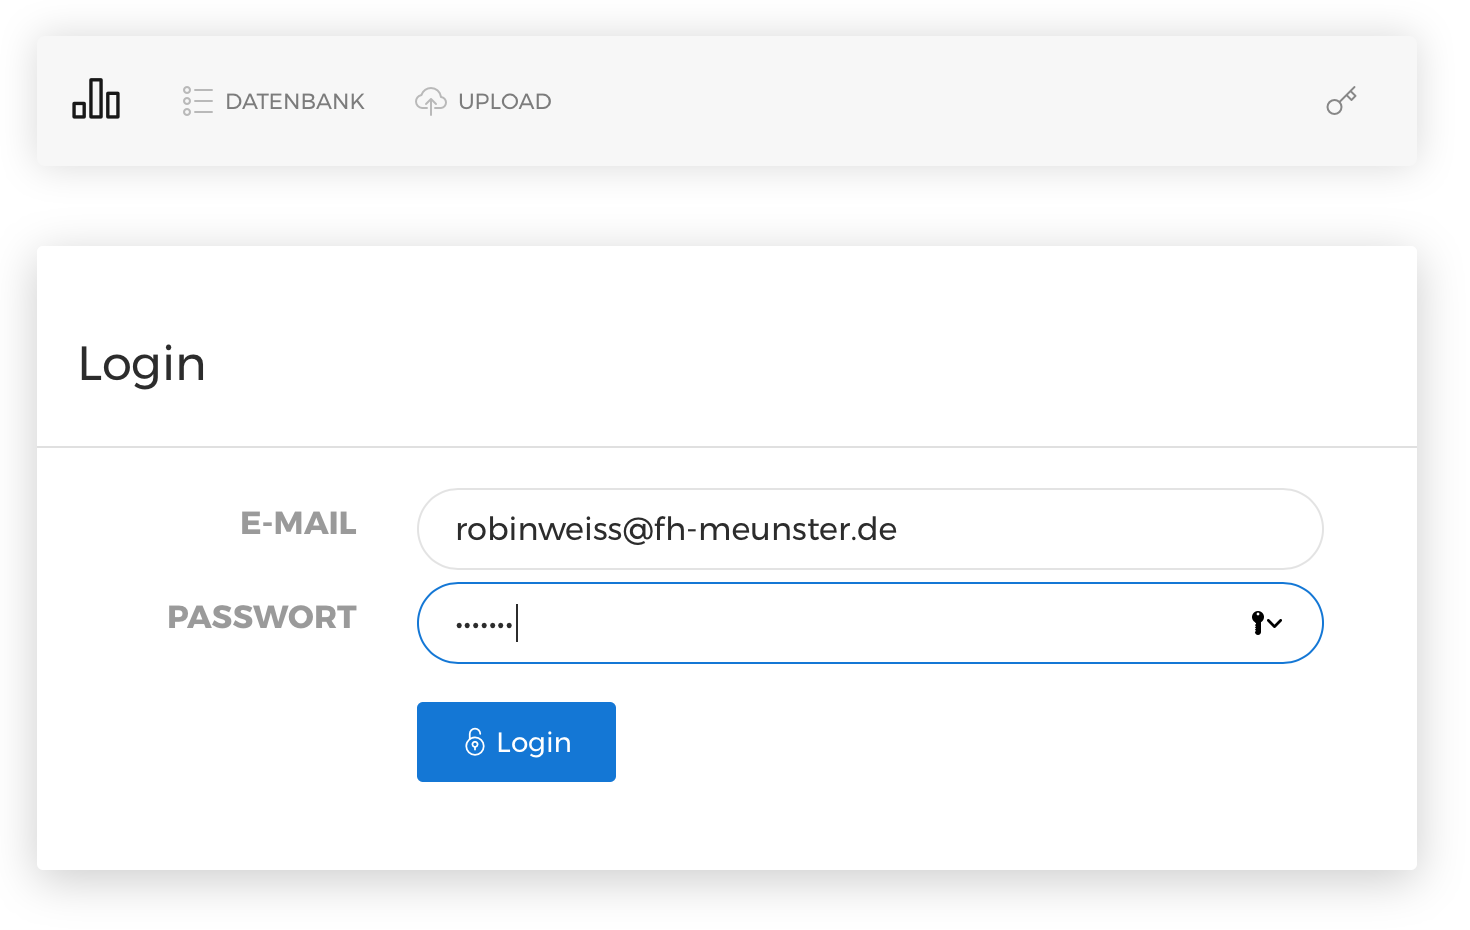
\includegraphics[width=\textwidth]{Figures/login}
\caption{Login-View}
\label{fig:login}
\end{figure}

\section{Dashboard}

Nach dem Login wird man zum Dashboard-View weitergeleitet. Dort wird der Name des Users sowie seine Rolle mit der er eingeloggt ist angezeigt, wie in Abbildung \ref{fig:dashboard}. Gleichzeitig ändern sich die Bedienelemente in der Navigationsleiste, über die man als Admin neue User hinzufügen, sich selbst ausloggen, oder die eigenen Nutzerdetails einsehen kann.

\begin{figure}
\centering
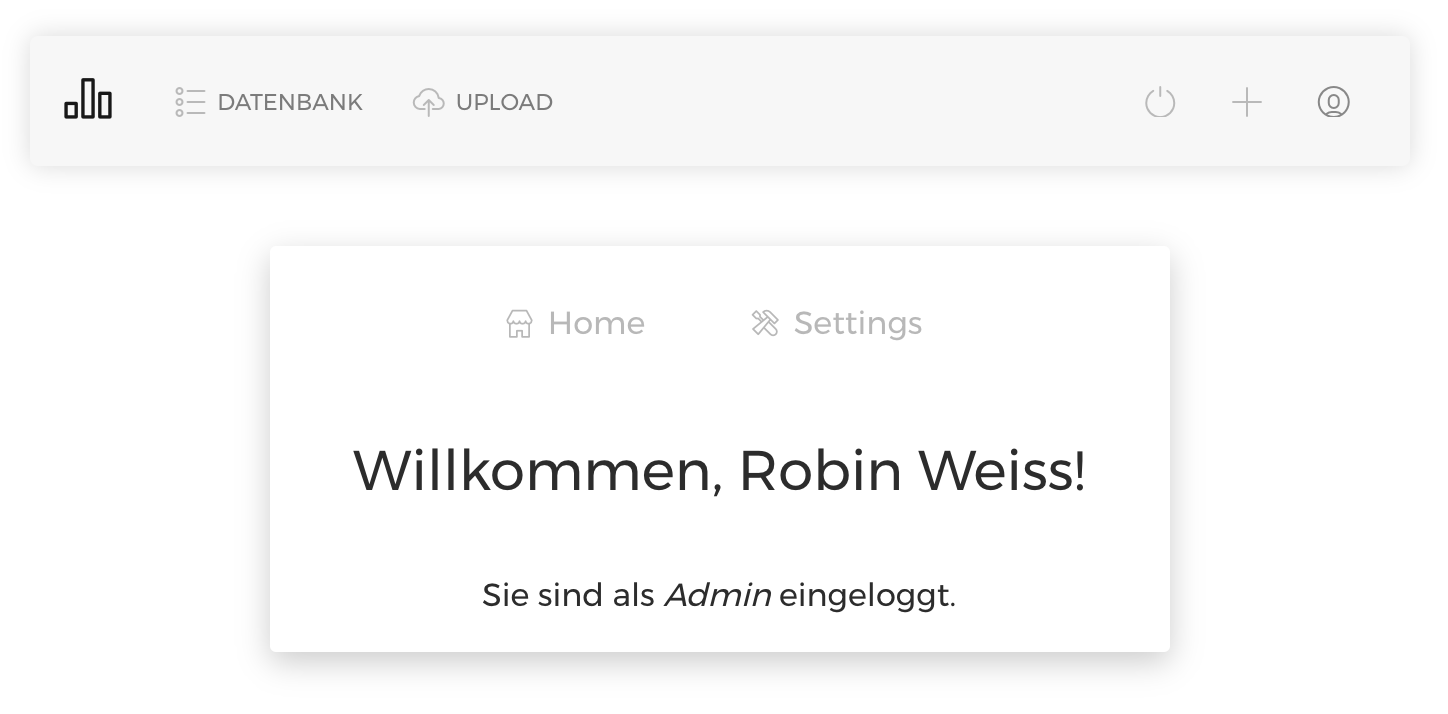
\includegraphics[width=\textwidth]{Figures/dashboard}
\caption{Dashboard-View}
\label{fig:dashboard}
\end{figure}

\section{Upload}

Klickt man nun über die Navigationsleiste am obigen Bildschirmrand auf Upload, gelangt man zum Upload-View, wie in Abbildung \ref{fig:upload} dargestellt, mit Hilfe dessen man per Drag-and-drop oder per Filebrowser Messdatenfiles zum Hochladen auswählen kann. Die Files werden in einer Warteschlange mit der jeweiligen Filegröße angezeigt und können einzeln oder alle nacheinander hochgeladen werden. Eine Progress-Bar zeigt jeweils Einzel- und Gesamtfortschritt des Uploads an.

\begin{figure}
\centering
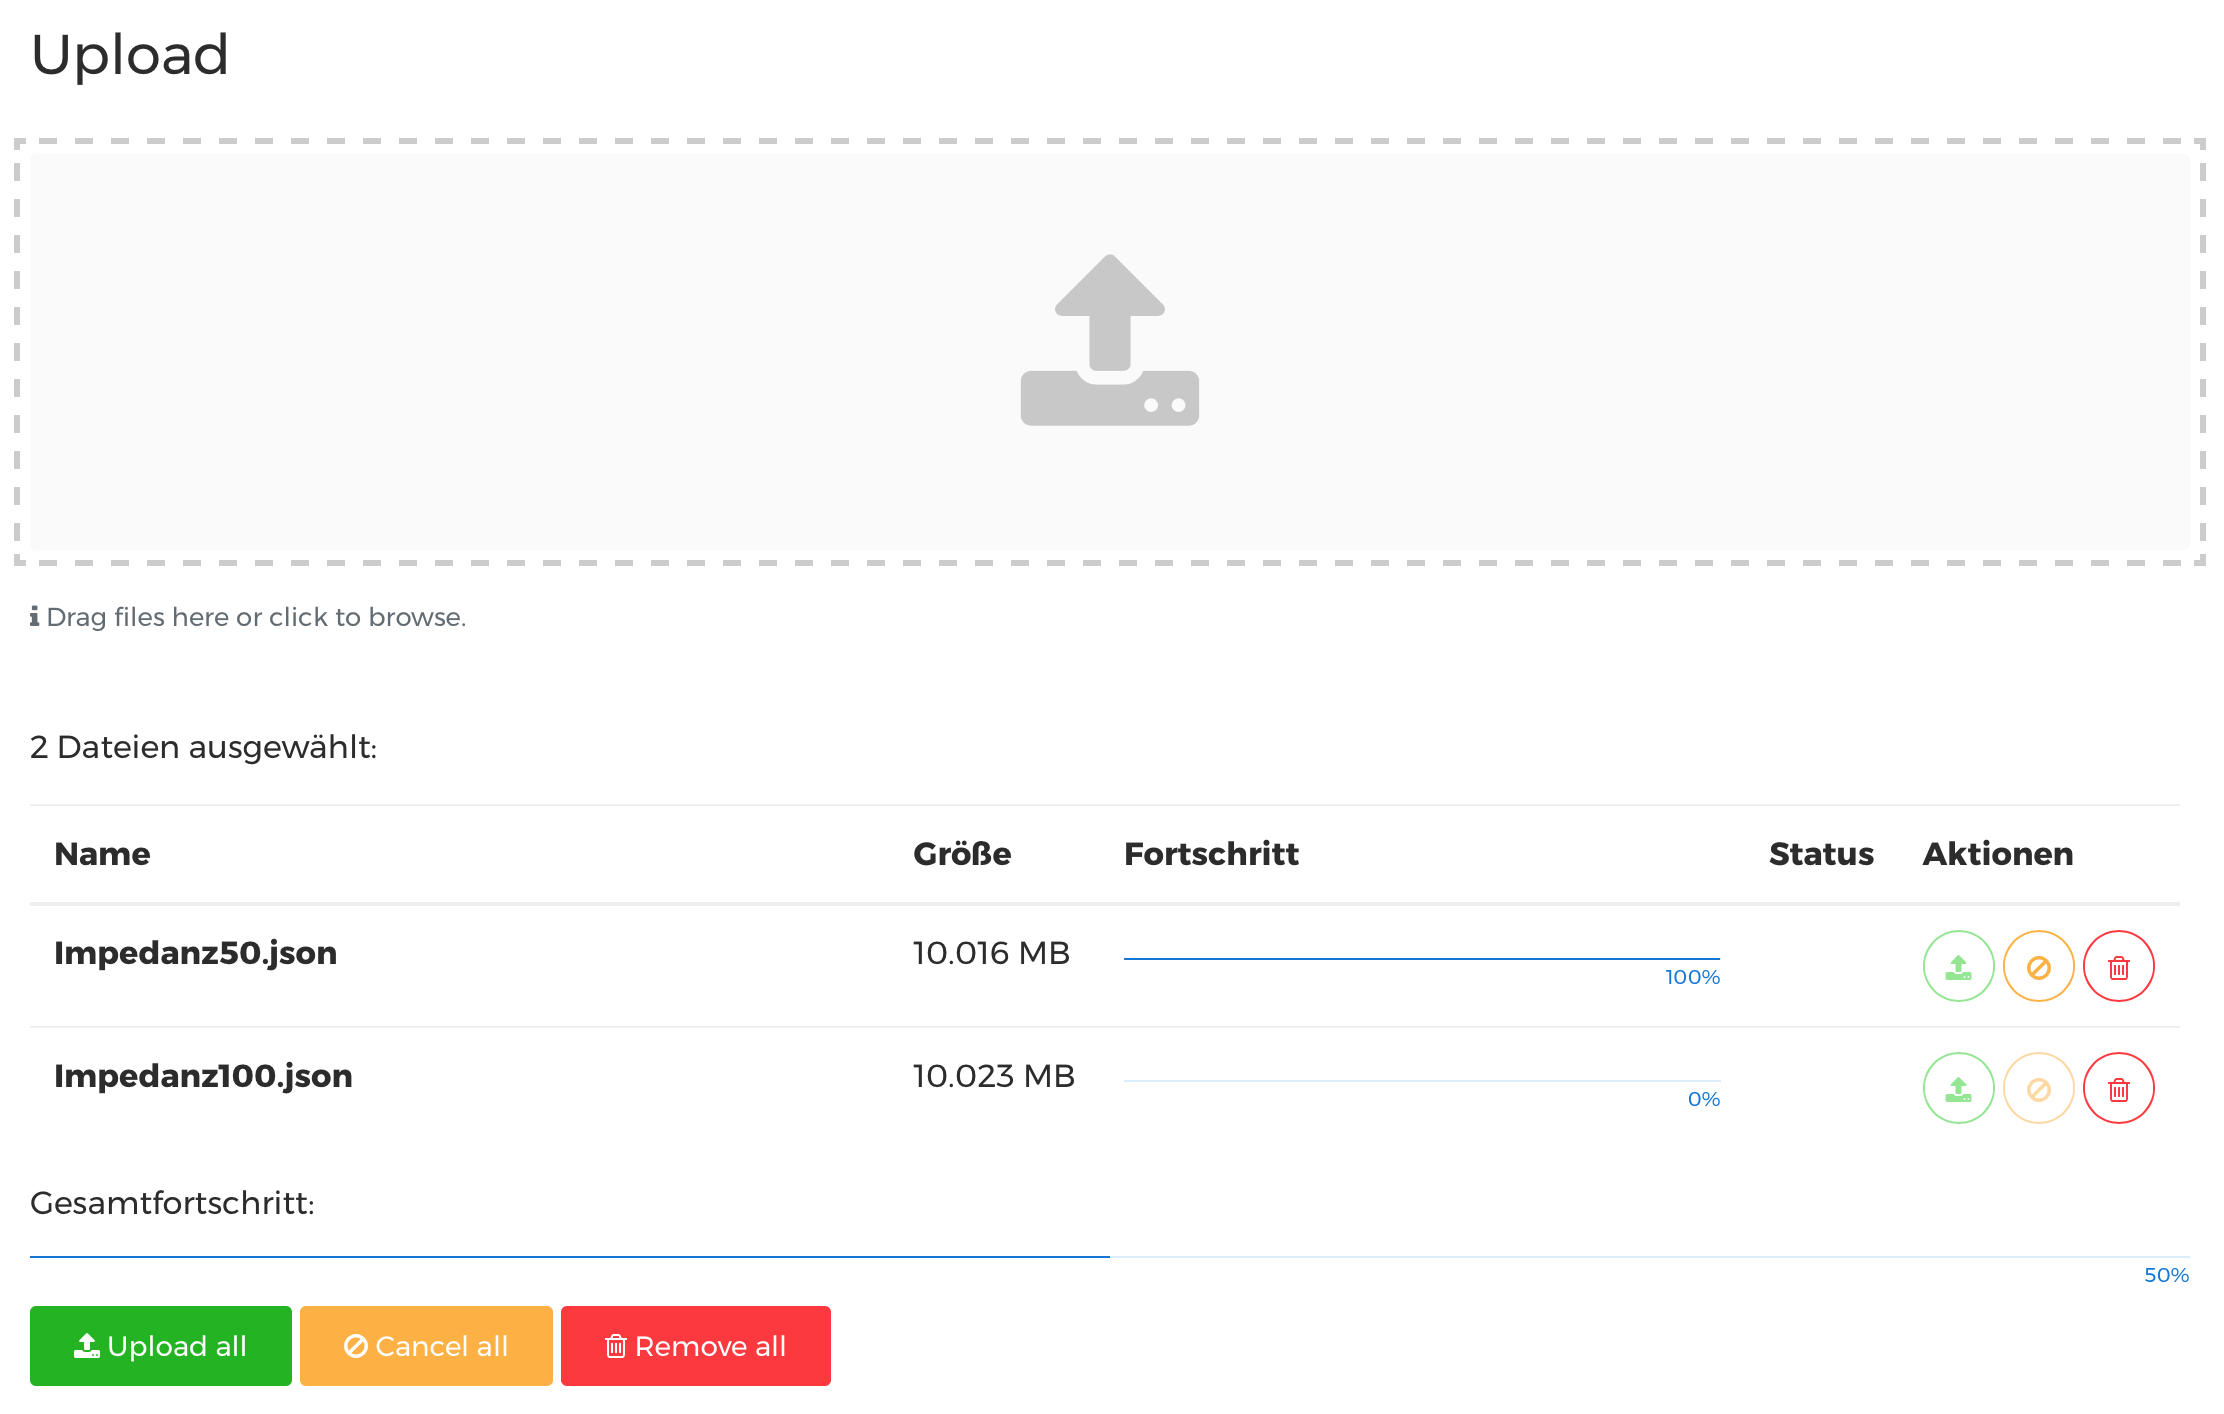
\includegraphics[width=\textwidth]{Figures/upload}
\caption{Upload-View}
\label{fig:upload}
\end{figure}


\section{Datenbank}

War der Upload erfolgreich wird man zur Datenbank weitergeleitet, in der, wie in Abbildung \ref{fig:messungen} zu sehen ist, durch Klicken auf die Seitenleiste eine Ansicht nach Systemen, Stacks, Zellen und Messungen ausgewählt werden kann. Die Ansicht mit den Messungen wird nach dem Upload automatisch ausgewählt. Hier finden sich alle Messungen in der Datenbank, sortiert in absteigender Reihenfolge, also mit den letzten Uploads ganz oben. Zusätzlich zum Namen der Messung, der mit dem Dateinamen initialisiert wird wenn es nicht anders im JSON-File spezifiziert ist, sind der Typ der Messung, also Zeitreihe oder Ortskurve, die Größe und das Datum der letzten Änderung in einer Tabelle dargestellt. Über drei Aktionsbuttons kann man die Details der Messung einsehen, sie bearbeiten oder löschen. Es werden jeweils 10 Messungen pro Seite dargestellt. Sind mehr als 10 Messungen in der Datenbank vorhanden, wird unter den Messungen eine Navigation mit Seitenzahlen eingeblendet.

\begin{figure}
\centering
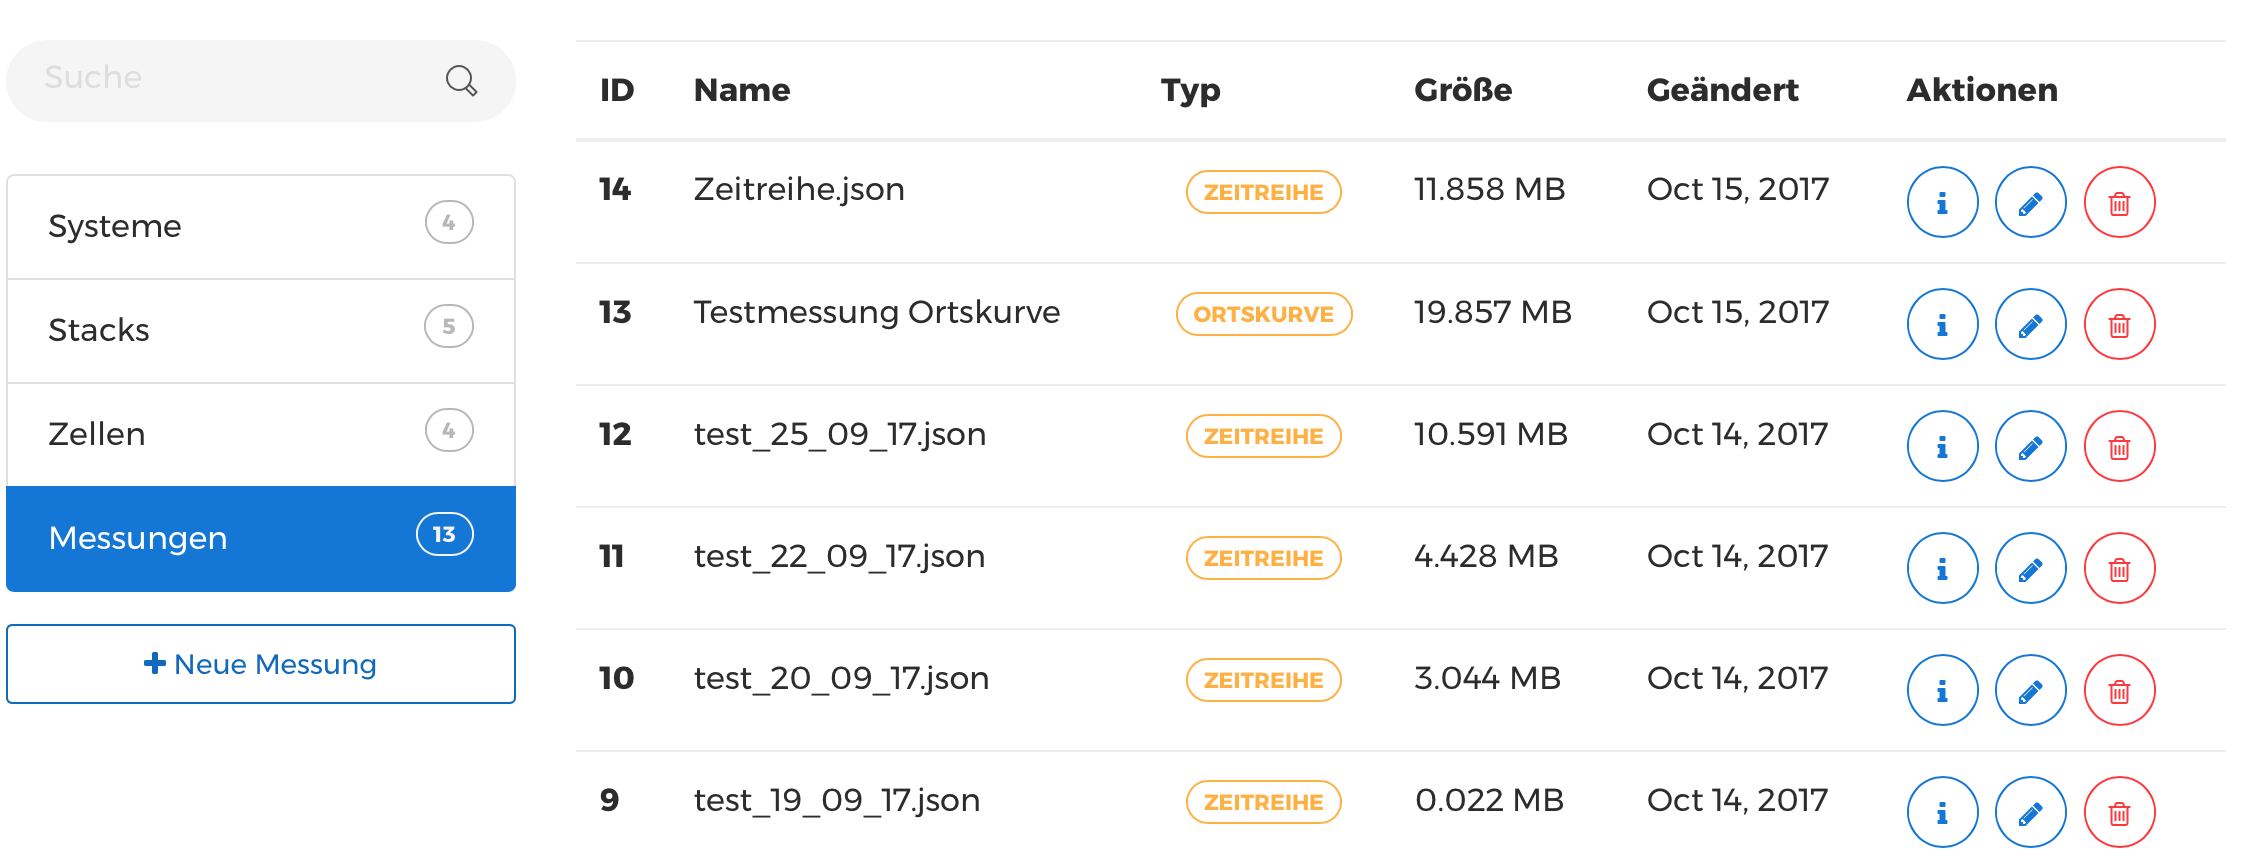
\includegraphics[width=\textwidth]{Figures/messungen}
\caption{Datenbank View mit Messungs-Ansicht}
\label{fig:messungen}
\end{figure}

Wählt man beispielsweise die Ansicht Stacks, wie in Abbildung \ref{fig:stacks} dargestellt, so werden die Stacks kachelweise mit Zusatzinformationen wie der Art der Verschaltung -- zum Beispiel Reihenschaltung -- und der Anzahl der zugehörigen Zellen angezeigt. Außerdem wird der Beschreibungstext und das Erstellungs- sowie letzte Änderungsdatum angezeigt. Über die oben beschriebenen Aktionsbuttons kann der Stack geändert oder gelöscht werden. Klickt man auf Details, gelangt man in die Detailansicht.

\begin{figure}
\centering
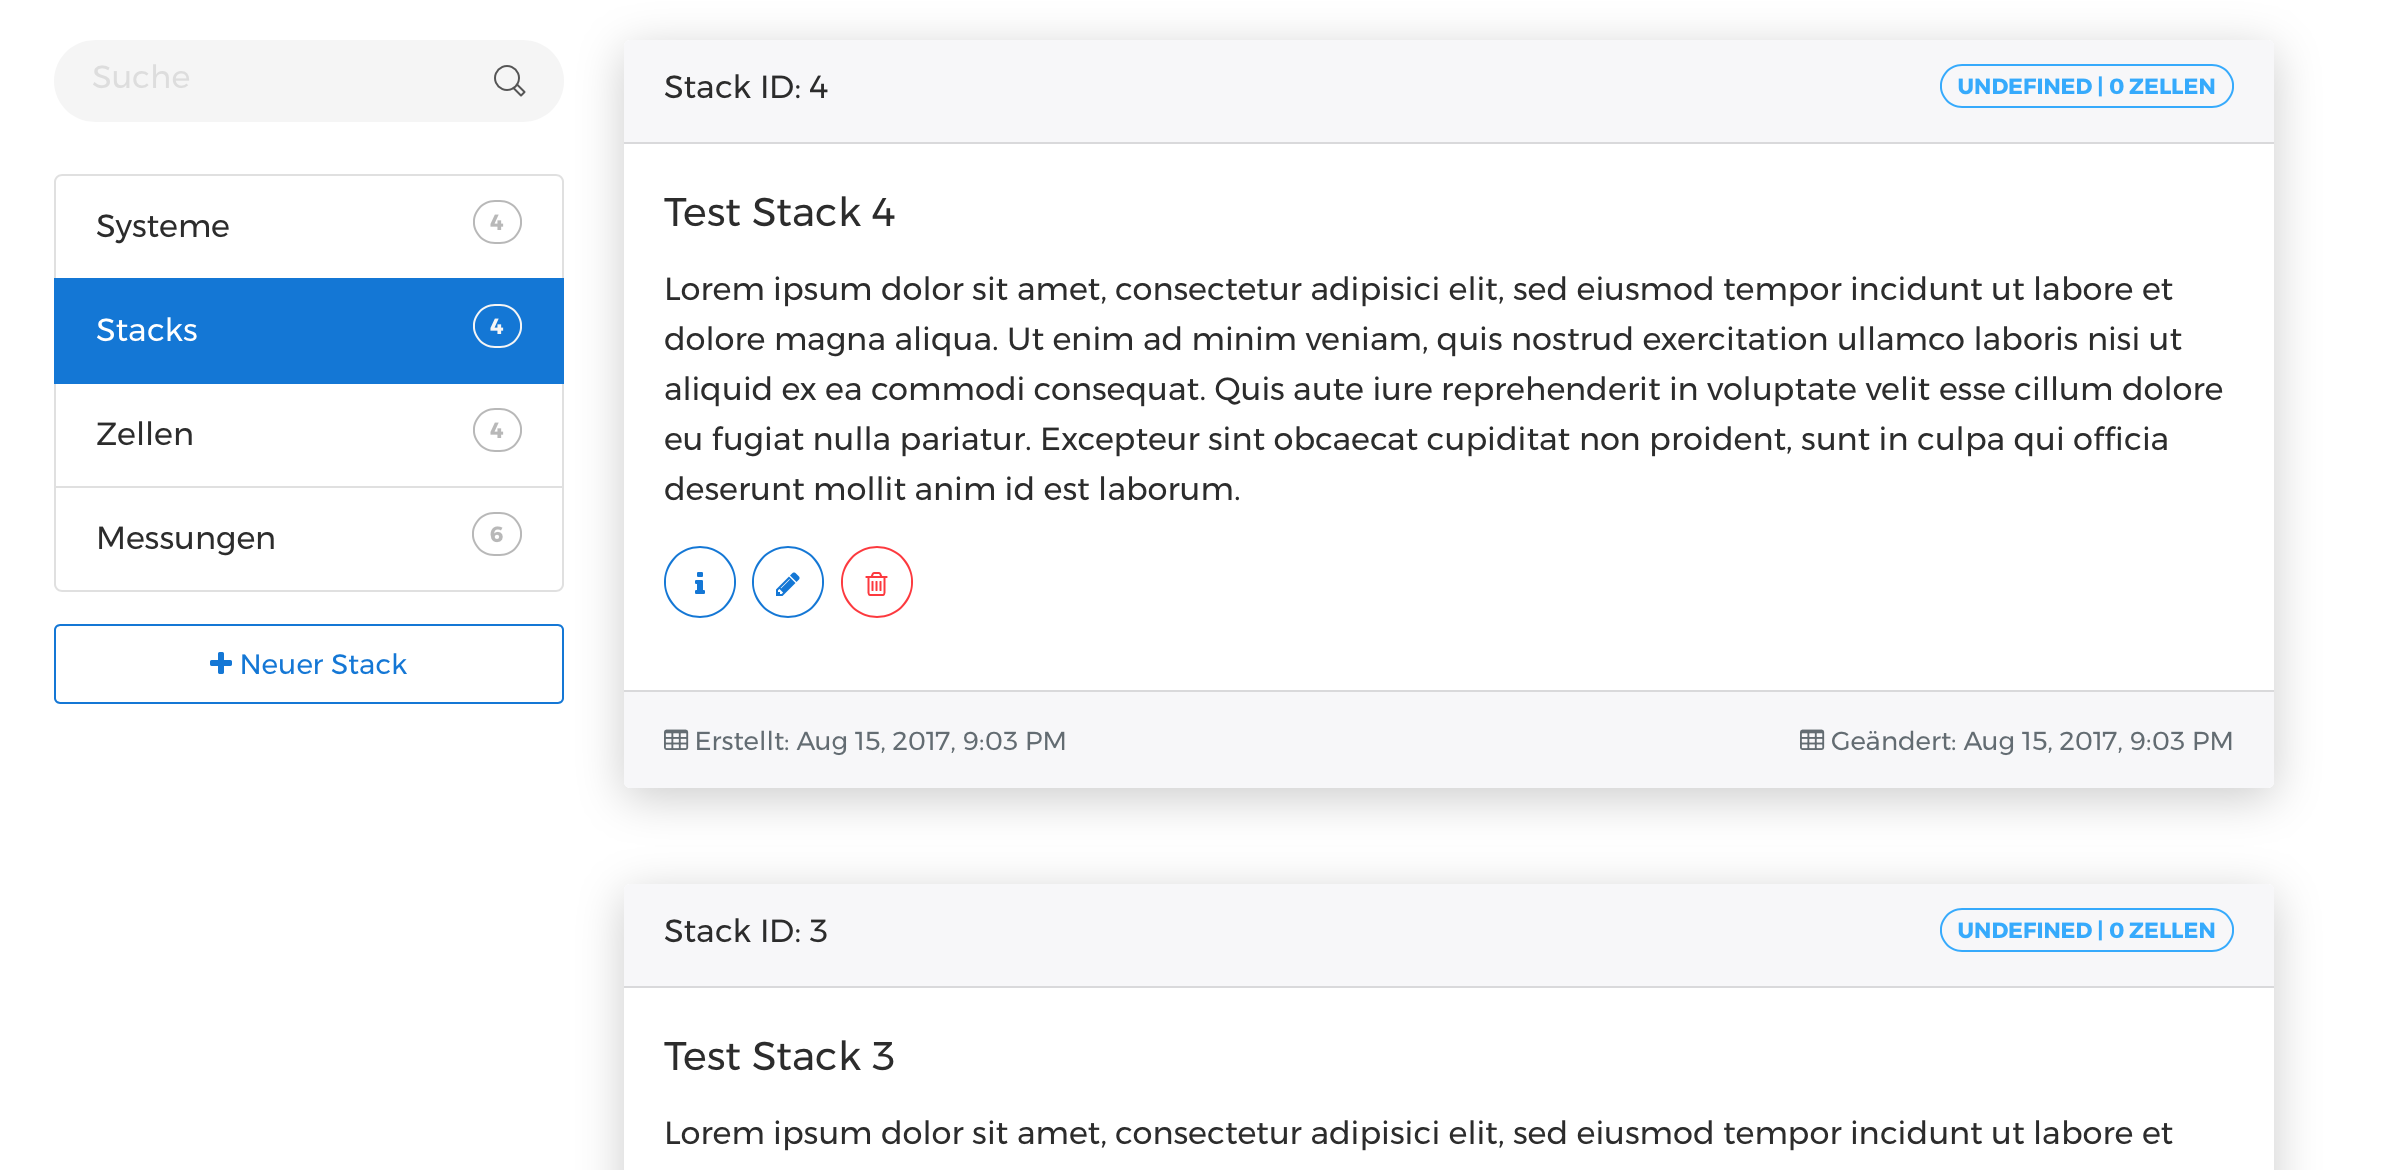
\includegraphics[width=\textwidth]{Figures/stacks}
\caption{Datenbank View mit Stack-Ansicht}
\label{fig:stacks}
\end{figure}

\section{Detialansicht}

Die Detailansicht in Abbildung \ref{fig:stack} zeigt wiederum die Beschreibung, die Markdownbefehle unterstützt, und listet die zu dem jeweiligen Stack gehörenden Messungen, unterteilt in Zeitreihen und Ortskurven, in einer Tabellenansicht ähnlich der Ansicht der Messungen in der Datenbank, auf.

\begin{figure}
\centering
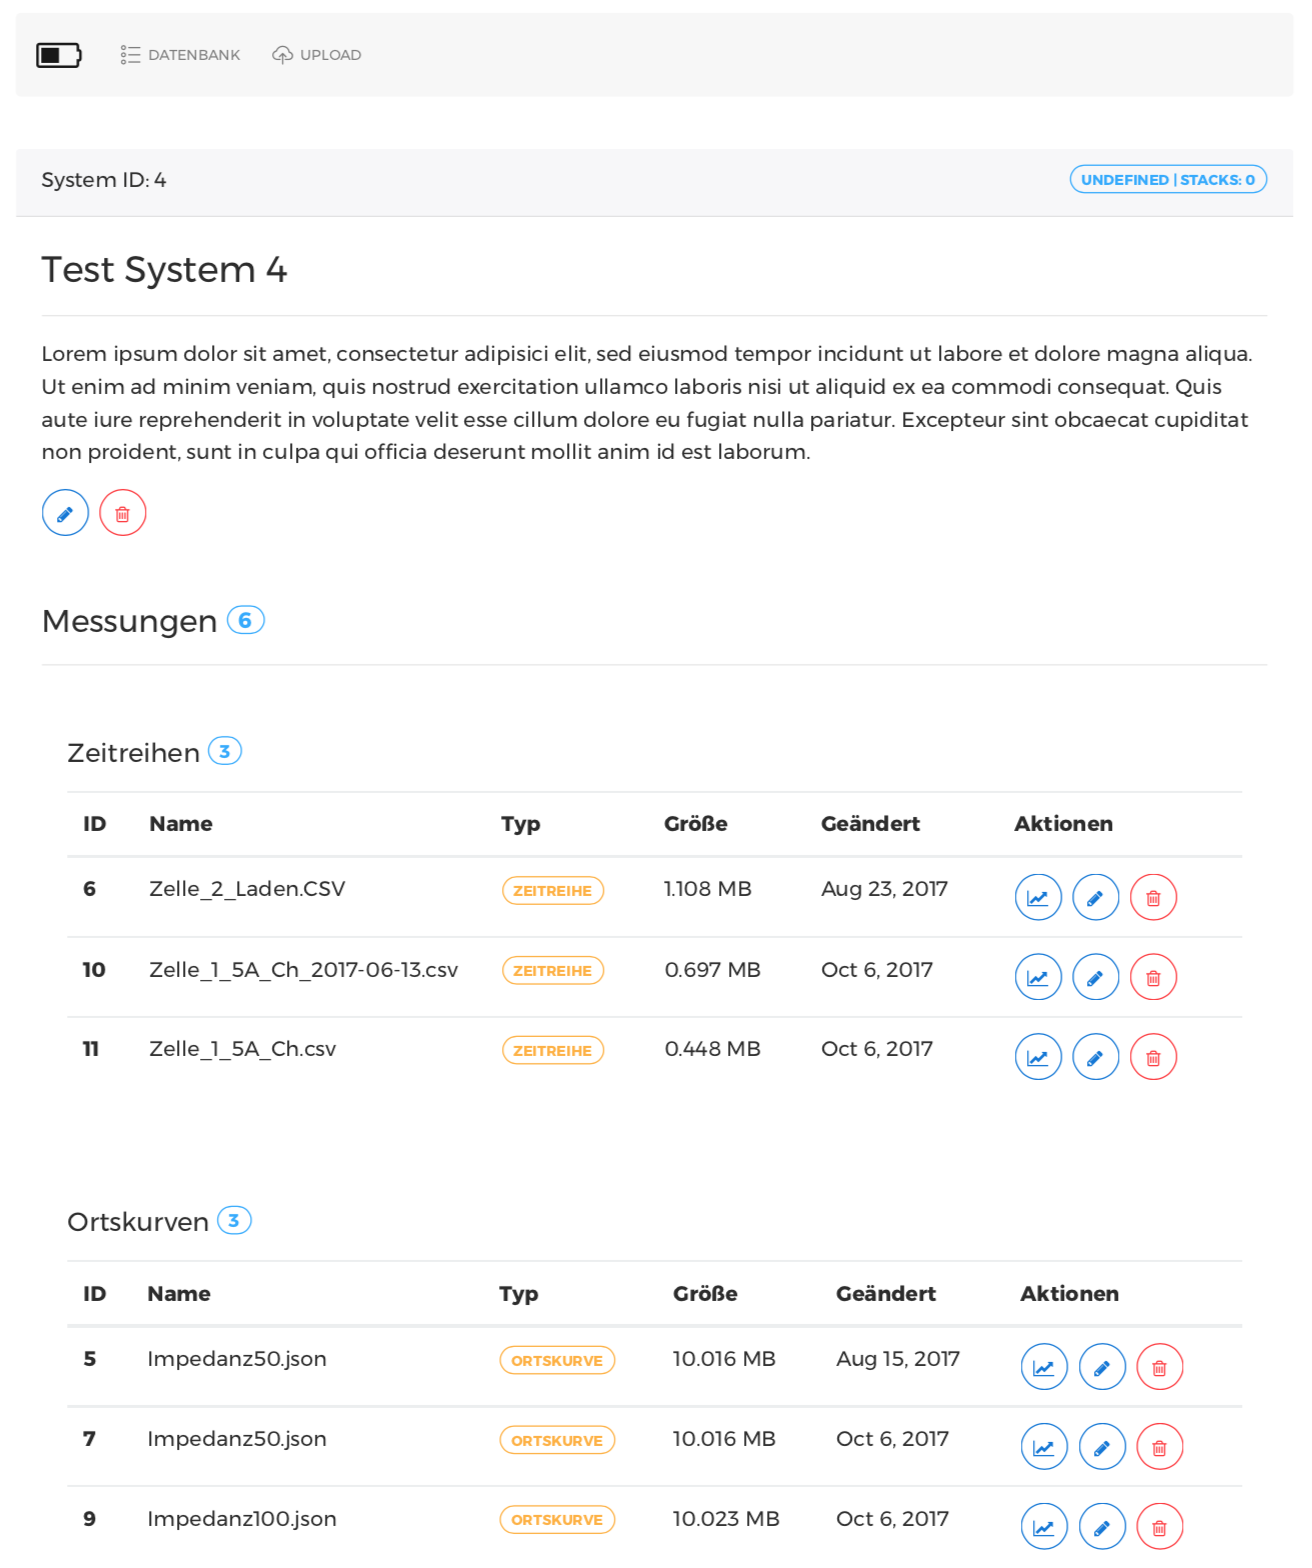
\includegraphics[width=\textwidth]{Figures/stack}
\caption{Stack-Detail-Ansicht}
\label{fig:stack}
\end{figure}

Klickt man nun auf eine Messung wird sie unter der entsprechenden Tabelle geplottet, wie in Abbildung \ref{fig:stackmessung} dargestellt. Der Klick auf eine der Messungen führt in die Detailansicht der jeweiligen Messung. Dort werden neben Details zur Messung auch jedes Mal die Messung als Plot dargestellt.

\begin{figure}
\centering
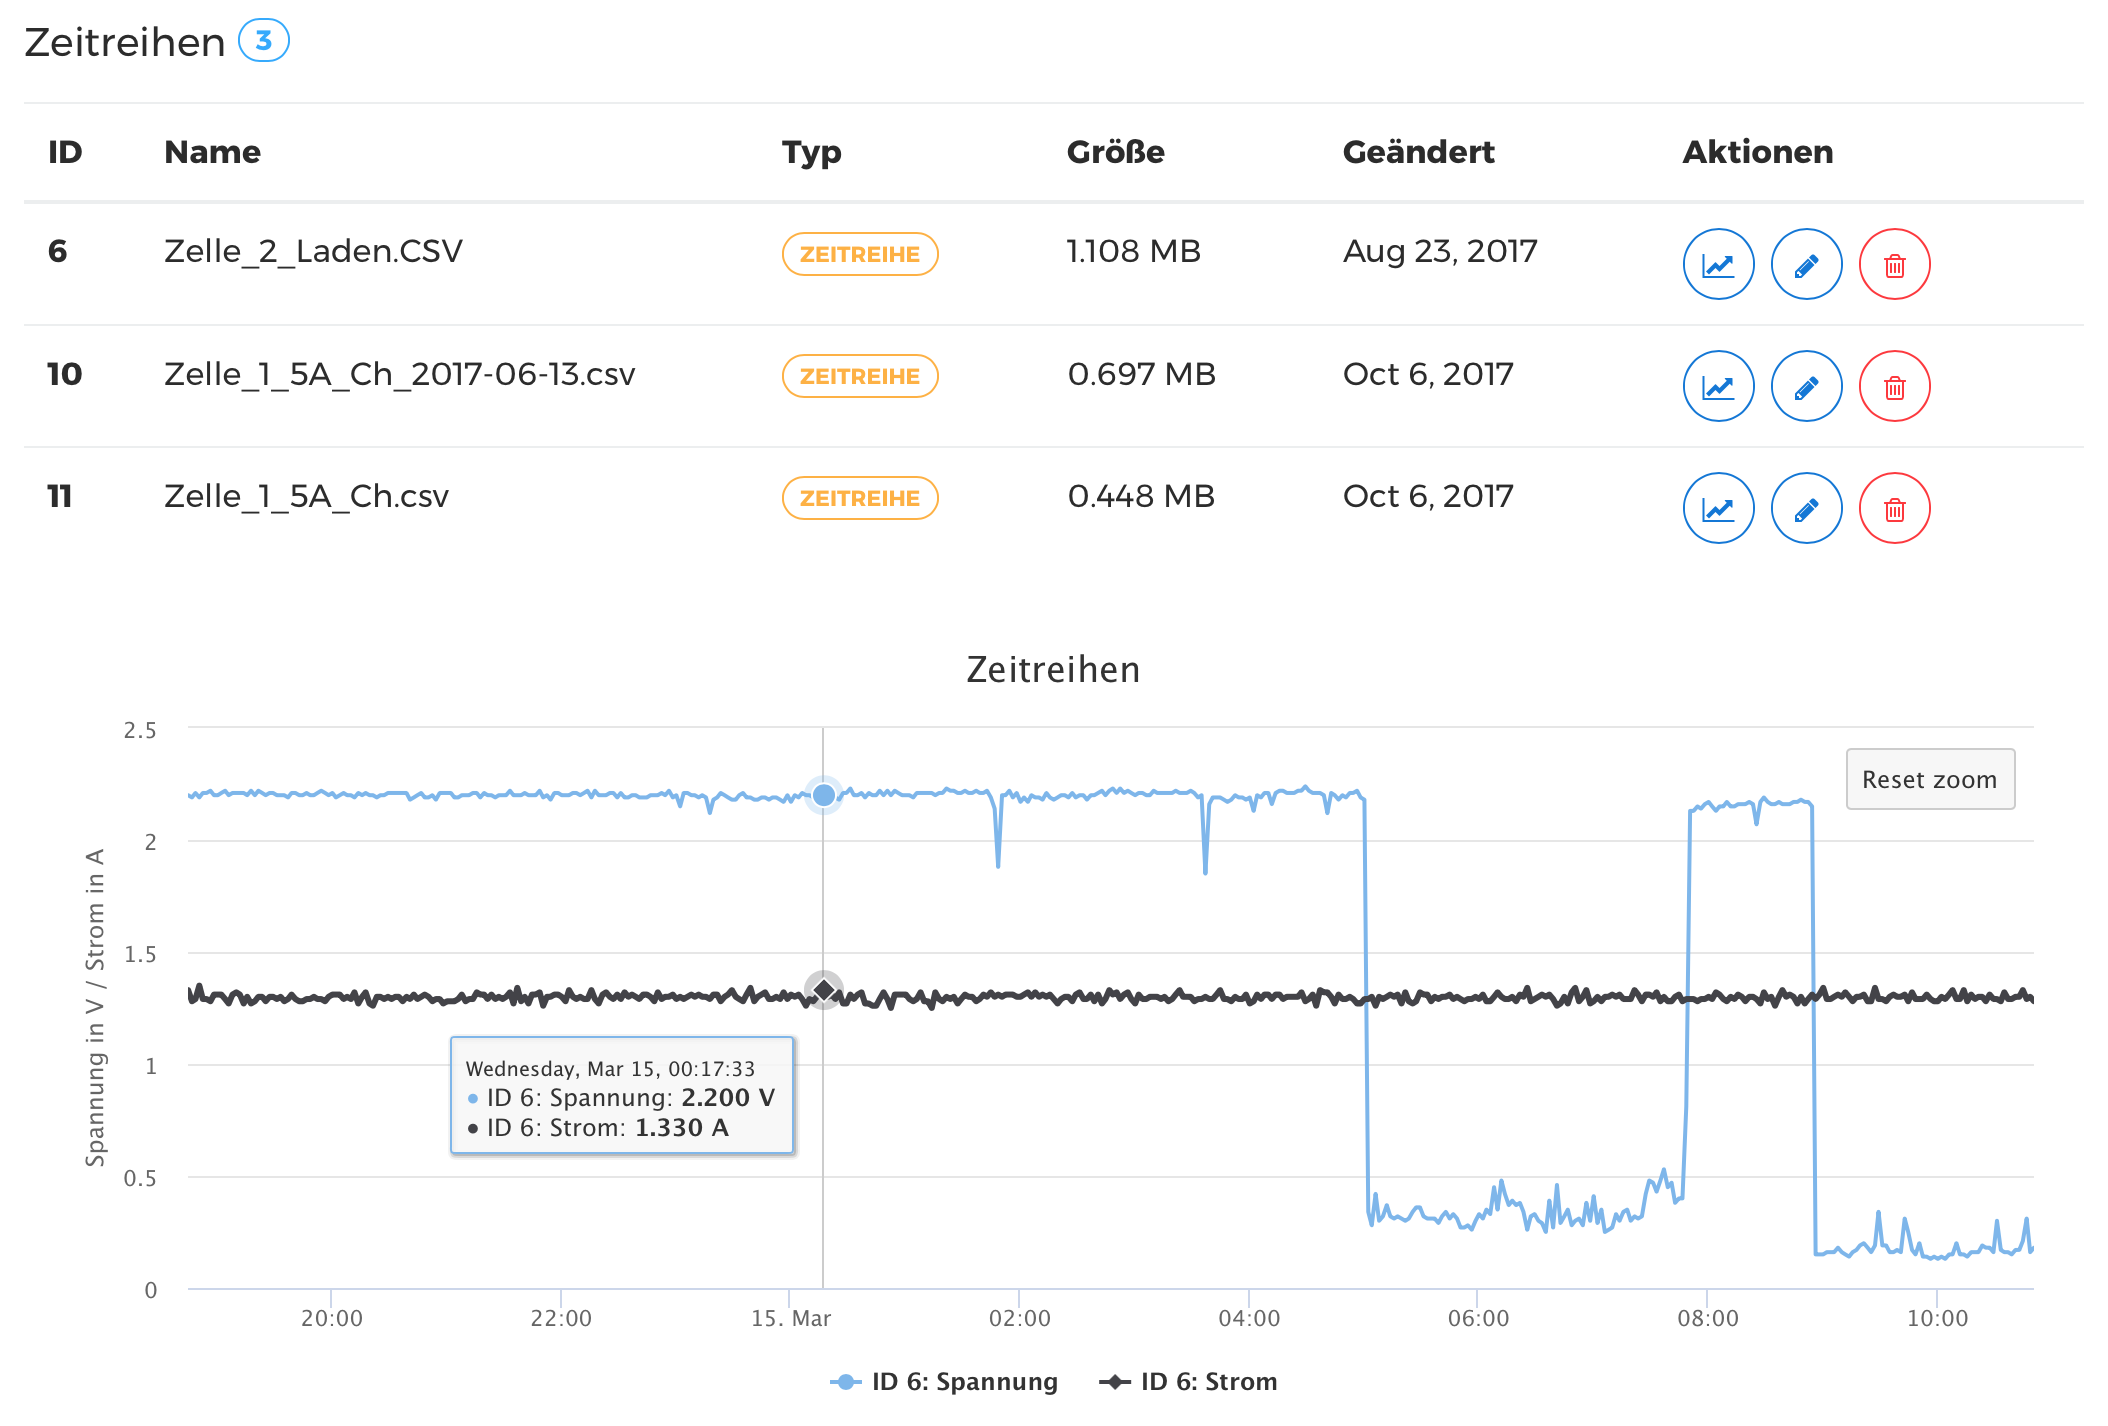
\includegraphics[width=\textwidth]{Figures/stackmessung}
\caption{Stackmessung}
\label{fig:stackmessung}
\end{figure}

\section{Plots}

Zeitreihen sind wie bei allen anderen Plots zoombar, wie in Abbildung \ref{fig:zoomvorher} (vorher) und Abbildung \ref{fig:zoomnachher} (nachher) dargestellt. Die Messdaten werden automatisch vom Server nachgeladen um den Plot mit einer höheren Auflösung darzustellen.

\begin{figure}
\centering
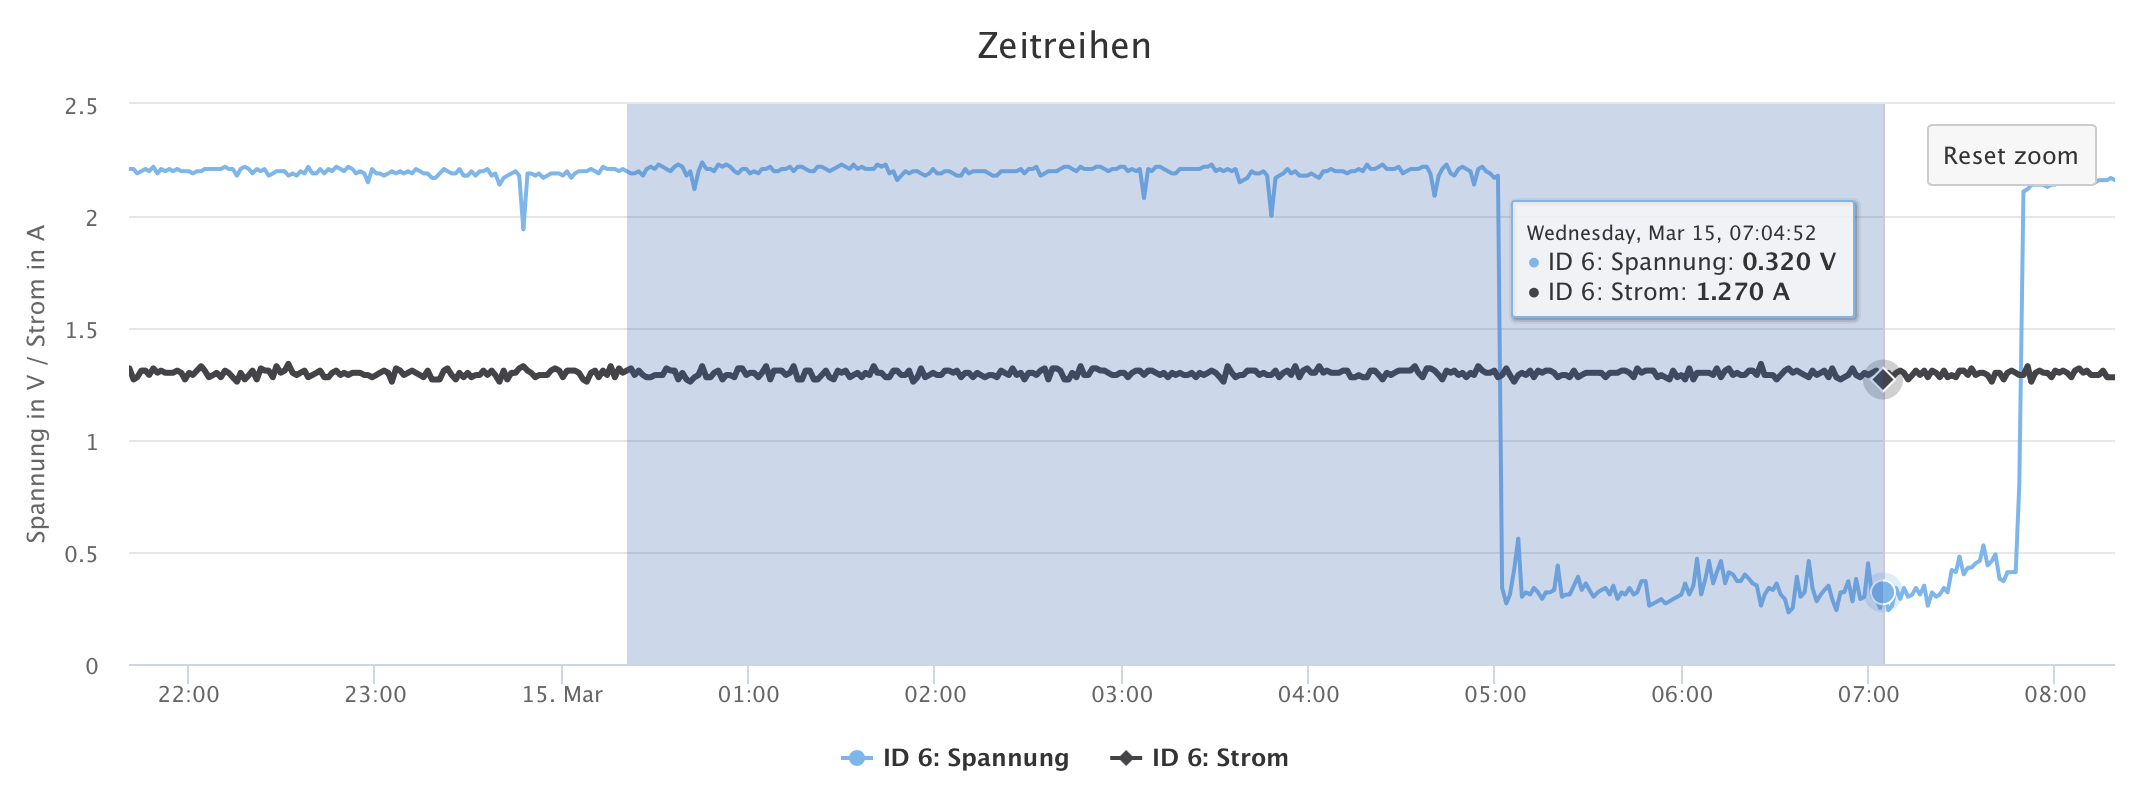
\includegraphics[width=\textwidth]{Figures/zoomvorher}
\caption{Zoom-Funktion vorher}
\label{fig:zoomvorher}
\end{figure} 

\begin{figure}
\centering
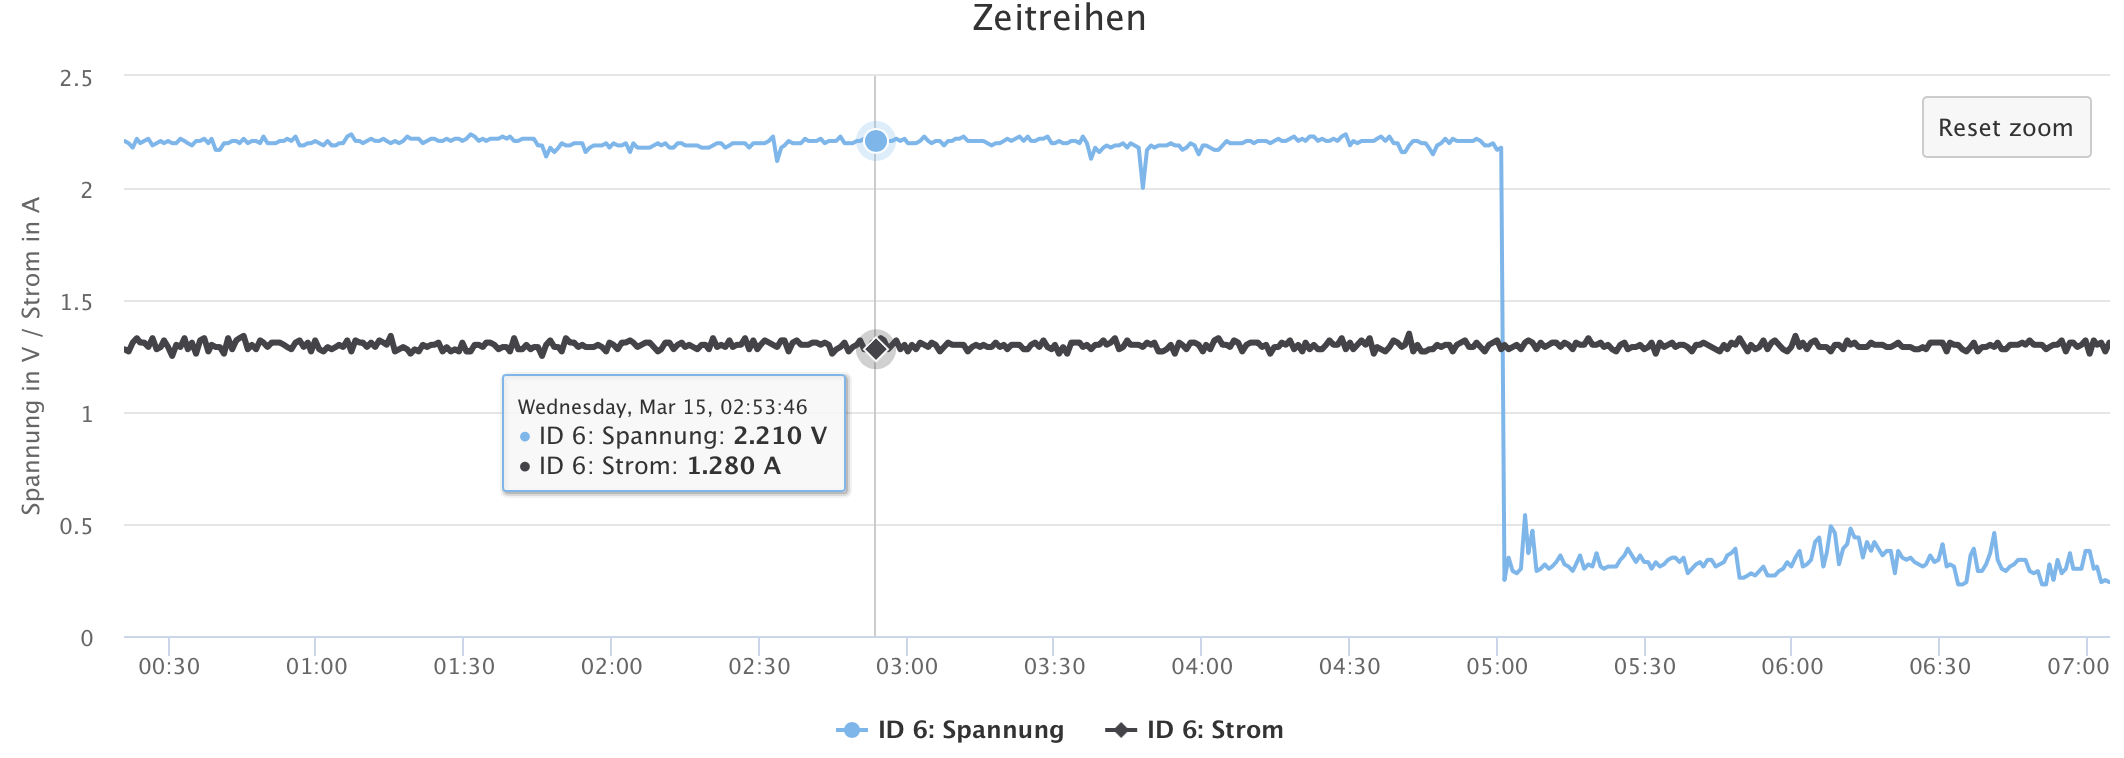
\includegraphics[width=\textwidth]{Figures/zoomnachher}
\caption{Zoom-Funktion nachher}
\label{fig:zoomnachher}
\end{figure} 

Bei Zeitreihen mit unterschiedlichen Größen können einzelne Zeitreihen durch Klick auf die Legende ein- und ausgeblendet werden um sie so vergrößert darzustellen, wie in Abbildung \ref{fig:legendeaktiviert} (Ladung aktiviert) und \ref{fig:legendedeaktiviert} (Ladung deaktiviert) dargestellt. Die Skalierung erfolgt automatisch.

\begin{figure}
\centering
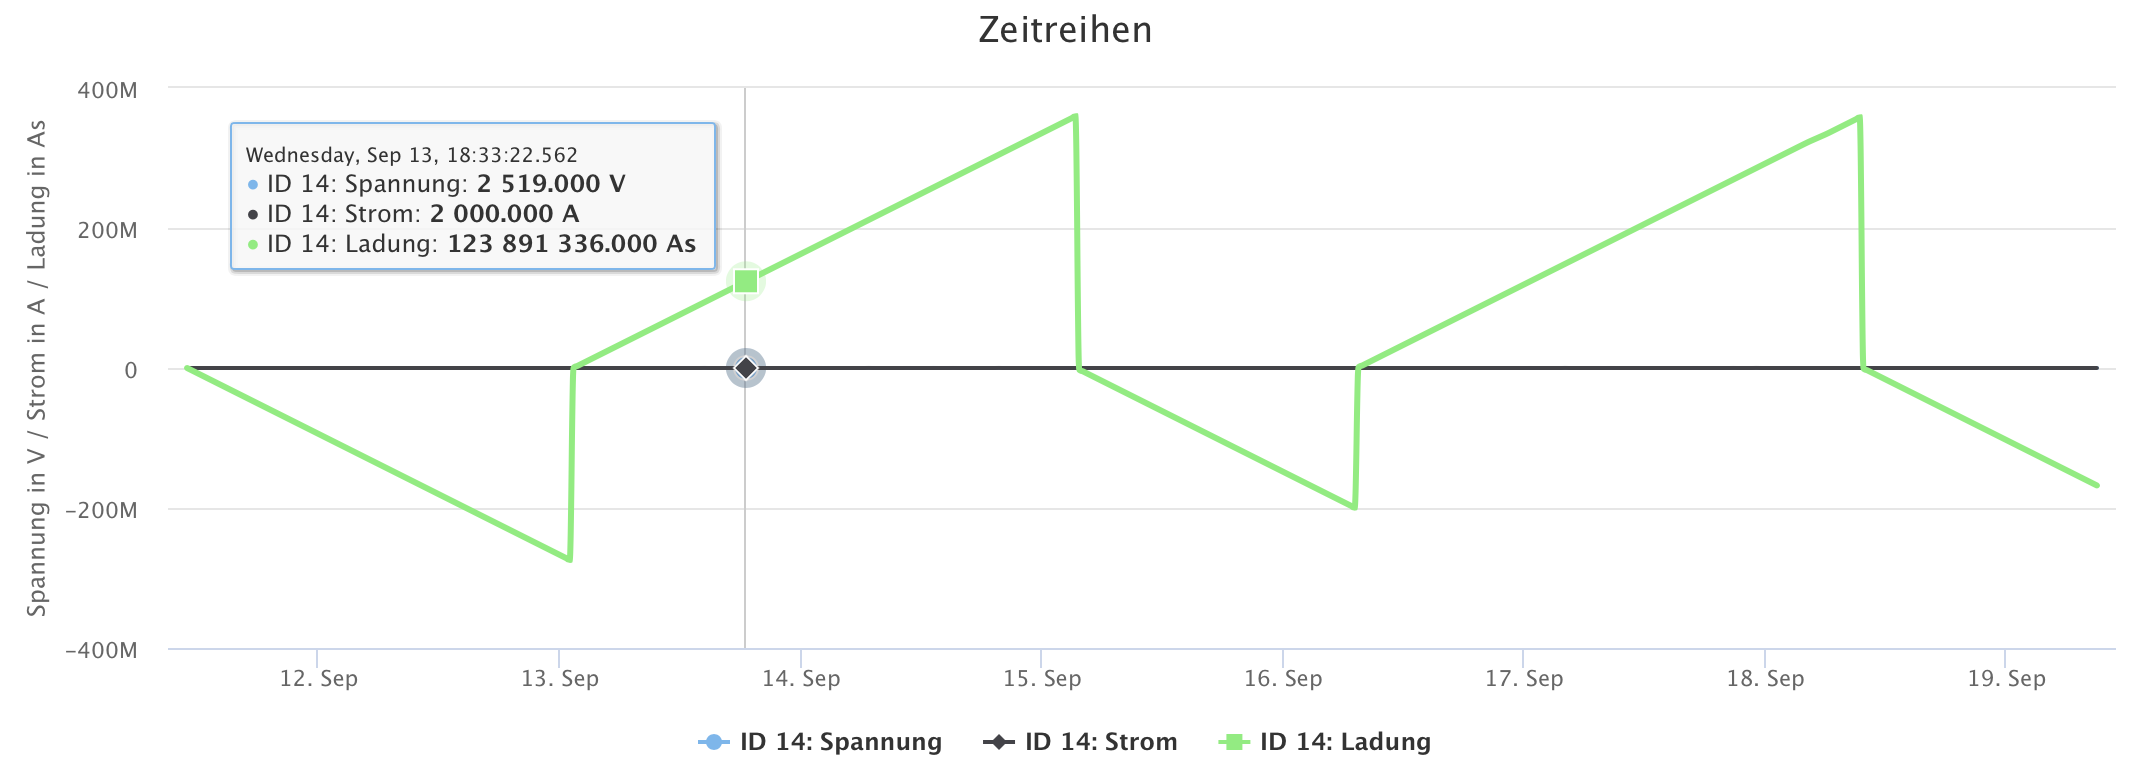
\includegraphics[width=\textwidth]{Figures/legendeaktiviert}
\caption{Ladungsplot aktiviert}
\label{fig:legendeaktiviert}
\end{figure} 

\begin{figure}
\centering
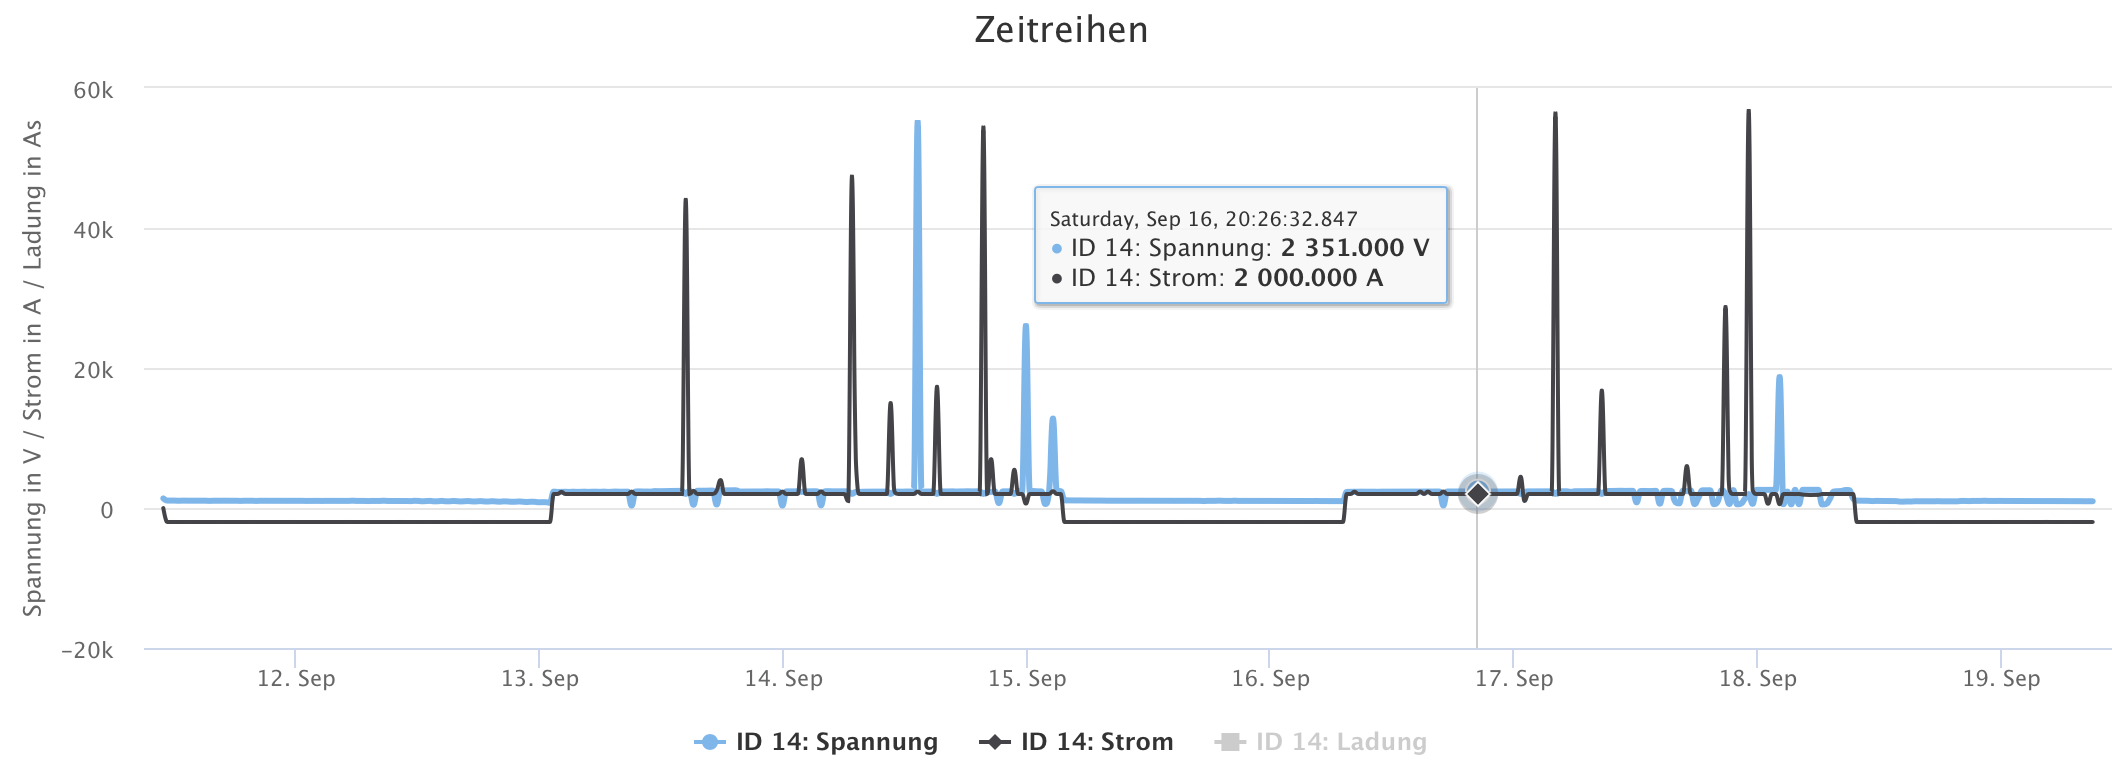
\includegraphics[width=\textwidth]{Figures/legendedeaktiviert}
\caption{Ladungsplot deaktiviert}
\label{fig:legendedeaktiviert}
\end{figure} 


Ein Plot einer Impedanzmessung ist in Abbildung \ref{fig:ortskurve} dargestellt. Die Koordinaten in der komplexen Ebene, wie auch die Frequenz sind am Cursor ablesbar.

\begin{figure}
\centering
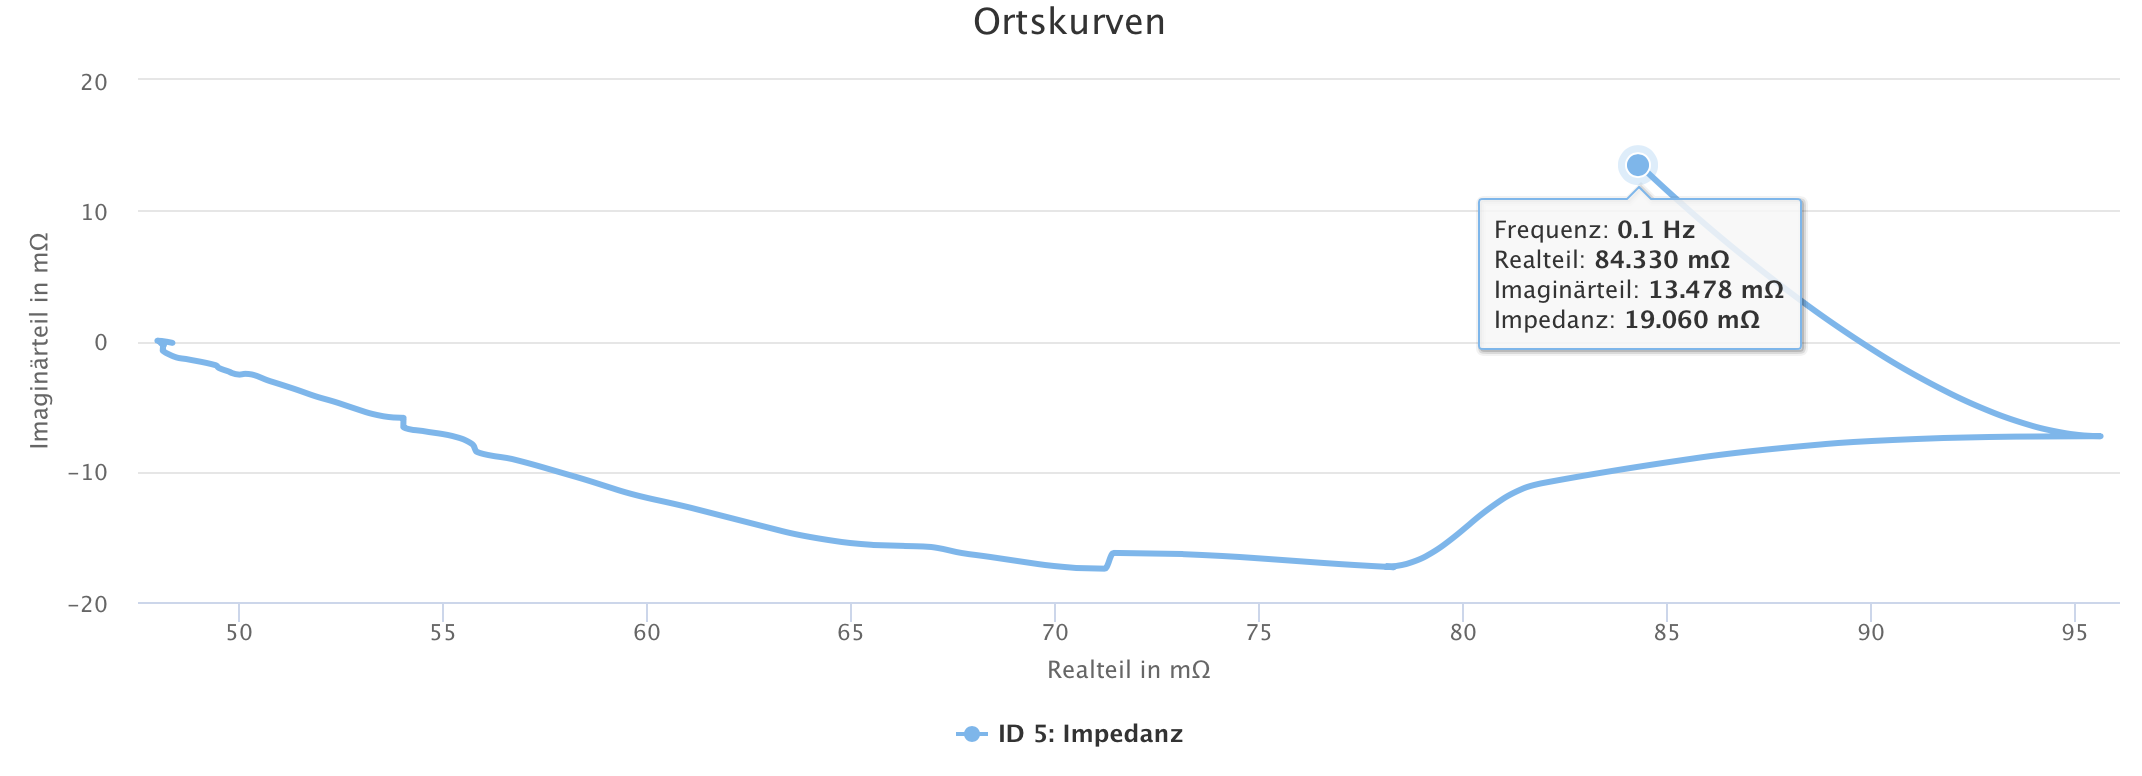
\includegraphics[width=\textwidth]{Figures/ortskurve}
\caption{Detailansicht einer Ortskurve}
\label{fig:ortskurve}
\end{figure}

\section{Notifications}

Bearbeitet oder löscht man Datensätze, oder fügt man neue durch Hochladen hinzu, wird das Ergebnis in Form von Notifications bzw. Fehlermeldungen im oberen rechten Bildschirmrand angezeigt. Dies ist in Abbildung \ref{fig:notifications} einmal für beide Fälle dargestellt.

\begin{figure}
\centering
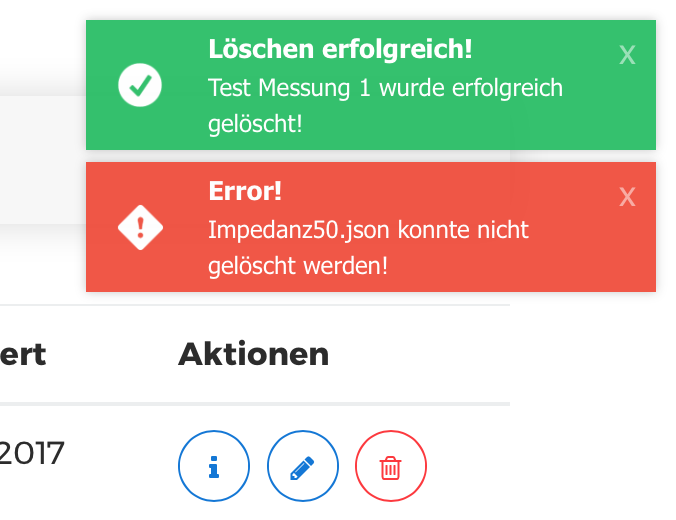
\includegraphics[width=0.5\textwidth]{Figures/notifications}
\caption{Notifications}
\label{fig:notifications}
\end{figure}

\section{Registrierung}

Neue Nutzer können nur durch bereits eingeloggte Nutzer mit Admin-Rechten hinzugefügt werden. Dafür kann man am oberen rechten Bildschirmrand auf das Plus klicken und gelangt zum Register-View, wie in Abbildung \ref{fig:register} dargestellt. Durch eintragen einer anderen Rolle, wir zum Beispiel "Mitarbeiter", erhält der neue Nutzer keine Admin-Rechte und kann so auch keine neuen Nutzer hinzufügen.

\begin{figure}
\centering
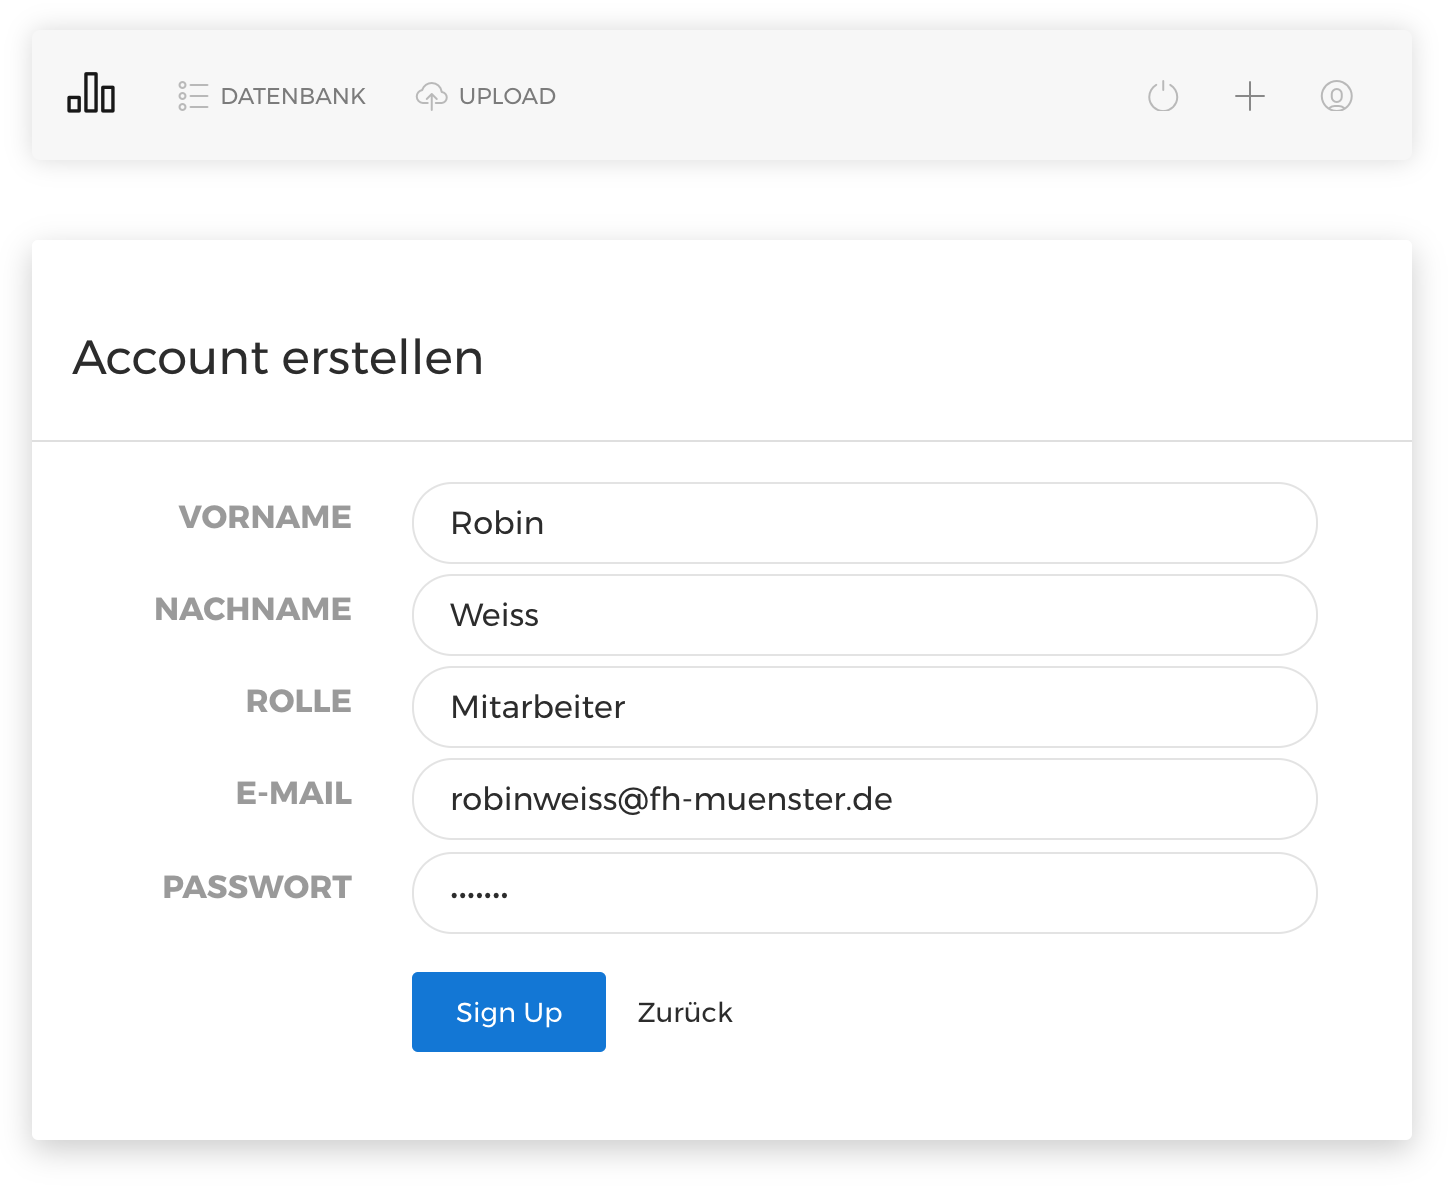
\includegraphics[width=\textwidth]{Figures/register}
\caption{Register-View}
\label{fig:register}
\end{figure}

